\documentclass[11pt,a4paper]{article}

\usepackage[margin=2.1cm]{geometry}
\usepackage{amsmath,amssymb,mathtools}
\usepackage{enumitem}
\usepackage{booktabs}
\usepackage{array}
\usepackage{longtable}
\usepackage{tabularx}
\usepackage{tikz}
\usetikzlibrary{automata,positioning,arrows.meta}
\usepackage{microtype}
\usepackage{setspace}
\usepackage[hidelinks]{hyperref}
\usepackage{fancyhdr}
\usepackage{xcolor}

\setstretch{1.12}
\setlength{\parskip}{0.32em}
\setlength{\parindent}{0pt}

\newcommand{\eps}{\varepsilon}
\newcommand{\lang}[1]{L(#1)}
\newcommand{\set}[1]{\{#1\}}
\newcommand{\powerset}[1]{\mathcal{P}(#1)}
\newcolumntype{L}[1]{>{\raggedright\arraybackslash}p{#1}}

\pagestyle{fancy}
\fancyhf{}
\setlength{\headheight}{14pt}
\lhead{MTL783}
\rhead{Sipser Ch.~1--2 problem-solving}
\cfoot{\thepage}

\title{\textbf{Sipser Chapters 1 and 2}\\[0.35em]
\large Problem-solving guide for exam constructions}
\author{Based on \emph{Introduction to the Theory of Computation},\\
3rd edition, Michael Sipser}
\date{}

\begin{document}
\maketitle

\noindent
This is \textbf{not} a chapter summary. It answers one question:

\begin{quote}
If an exam problem comes from Sipser Chapter~1 or~2, what kind of problem is
it, how do I recognise it, and what exact method do I use?
\end{quote}

Sipser's own distinction is used throughout: \textbf{Exercises} test definitions
and standard constructions; \textbf{Problems} need more ingenuity. Selected
solutions in the book are marked \textbf{Book}. Solutions constructed here are
marked \textbf{Constructed here}.

\tableofcontents
\newpage

\section*{How to use this guide}
\addcontentsline{toc}{section}{How to use this guide}

\begin{enumerate}[leftmargin=1.4em]
  \item Read the exam question and match it to a type in the
        \hyperref[sec:quickref]{Question $\to$ Method} table.
  \item Follow the numbered method for that type. Do not invent a new
        construction if Sipser already gives one.
  \item Check the \textbf{important cases} and \textbf{common mistake}
        before writing the answer.
\end{enumerate}

Sipser notation used throughout:
$M=(Q,\Sigma,\delta,q_0,F)$ for a DFA;
$\delta:Q\times\Sigma_\eps\to\powerset{Q}$ for an NFA, where
$\Sigma_\eps=\Sigma\cup\{\eps\}$;
$G=(V,\Sigma,R,S)$ for a CFG;
$P=(Q,\Sigma,\Gamma,\delta,q_0,F)$ for a PDA, with labels
$a,b\to c$ meaning ``read $a$, pop $b$, push $c$''.

%======================================================================
\part{Chapter 1: Regular languages}
%======================================================================

\section{Reading and describing a finite automaton}
\label{type:dfa-read}

\subsection{Trace a DFA or NFA on a string}

\textbf{What they can ask.}
\begin{itemize}[nosep]
  \item What is the start state / set of accept states?
  \item What sequence of states does the machine go through on $w$?
  \item Does the machine accept $w$? Does it accept $\eps$?
\end{itemize}

\textbf{How to recognize it.}
A diagram or $5$-tuple is given, and the question is about \emph{that}
machine, not about inventing a new one. Sipser Ex.~1.1 is the prototype.

\textbf{Method.}
\begin{enumerate}
  \item Start at the unique start state.
  \item For a DFA: from the current state, follow the unique arrow labelled
        with the next input symbol. Record the state after every symbol.
  \item Accept iff the state after the last symbol is in $F$.
  \item $\eps$ is accepted iff the start state itself is an accept state.
  \item For an NFA: a string is accepted if \emph{some} computation path
        ends in $F$. Track the \emph{set} of possible states after each
        symbol, including $\eps$-closure.
\end{enumerate}

\textbf{Important cases.}
\begin{itemize}[nosep]
  \item $F=\varnothing$ accepts nothing, including $\eps$.
  \item A DFA always has exactly one transition for every $(q,a)$.
  \item An NFA may get stuck (no transition). That branch dies and rejects.
\end{itemize}

\textbf{Mini-example.}
Sipser Ex.~1.1 on $aabb$. \textbf{Book:} $M_1$ visits
$q_1,q_2,q_3,q_1,q_1$ and rejects; $M_2$ visits
$q_1,q_1,q_1,q_2,q_4$ and accepts. $M_1$ rejects $\eps$; $M_2$ accepts
$\eps$.

\textbf{Common mistake.}
Forgetting that acceptance is checked only \emph{after} the whole input is
read. Leaving an accept state mid-string does not accept.

\subsection{Formal description $\leftrightarrow$ state diagram}

\textbf{What they can ask.}
Give the $5$-tuple for a pictured machine, or draw the diagram of a
$5$-tuple / transition table. Sipser Ex.~1.2, 1.3.

\textbf{Method.}
\begin{enumerate}
  \item $Q$: every circle. $\Sigma$: every arrow label.
  \item $q_0$: the state with the incoming start arrow.
  \item $F$: double circles.
  \item $\delta$: one row per state, one column per symbol.
  \item Diagram from a table: one node per state, one arrow per table entry.
        Mark start and accept exactly as specified.
\end{enumerate}

\textbf{Mini-example.}
Sipser Ex.~1.2. \textbf{Book:}
$M_1=(\{q_1,q_2,q_3\},\{a,b\},\delta_1,q_1,\{q_2\})$ with
$\delta_1(q_1,a)=q_2$, $\delta_1(q_1,b)=q_1$, $\delta_1(q_2,a)=q_3$,
$\delta_1(q_2,b)=q_3$, $\delta_1(q_3,a)=q_2$, $\delta_1(q_3,b)=q_1$.

\textbf{Common mistake.}
Omitting a transition. A DFA diagram is illegal if some $(q,a)$ has no
arrow.

%======================================================================
\section{Constructing a DFA}
\label{type:dfa-design}

\subsection{The master method: finite memory}

This is Sipser's design method (p.~41). Almost every ``construct a DFA''
question is an instance of it.

\textbf{What they can ask.}
Give a state diagram / formal description of a DFA for a stated language.
Sipser Ex.~1.6 is the main bank of such questions.

\textbf{How to recognize it.}
The language is specified by a finite condition on the string seen so far:
parity, count up to a fixed $k$, last few symbols, a fixed pattern, a
modular residue, a Boolean combination of such conditions.

\textbf{Method.}
\begin{enumerate}
  \item Pretend you are the machine. You see one symbol at a time and must
        always be ready to accept or reject, because you do not know when
        the input ends.
  \item Ask: \emph{what finite information must I remember?} List the
        possible values of that information. Those become the states.
  \item Draw a transition for every state and every alphabet symbol, by
        asking how the remembered information updates.
  \item Start state $=$ the information after seeing $\eps$.
  \item Accept states $=$ those information-values for which the string
        seen so far is in the language.
\end{enumerate}

\textbf{Common mistake.}
Trying to remember the entire string. If the necessary information is
infinite (``how many $0$s so far, with no bound''), a DFA is impossible
and the language is not regular.

\subsection{DFA pattern catalogue}

Each row is a reusable state design. $\Sigma=\{0,1\}$ unless noted.

\subsubsection{Parity / even--odd}

Remember one bit.

\begin{center}
\begin{tabular}{@{}llp{7.4cm}@{}}
\toprule
Language & States & Transition idea \\
\midrule
odd number of $1$s & $q_{\mathrm{even}},q_{\mathrm{odd}}$ &
flip on $1$, stay on $0$; start even; accept odd \\
even length & $q_0,q_1$ & flip on every symbol; start $q_0$; accept $q_0$ \\
even $0$s and odd $1$s & four pair-states & product of two parity machines \\
\bottomrule
\end{tabular}
\end{center}

Sipser's own example (p.~41): odd number of $1$s.

\subsubsection{Contains a fixed substring}

Remember the longest prefix of the target that is also a suffix of the
text read so far.

\textbf{Sipser Example~1.21:} contains $001$. Four states:
haven't seen any of the pattern; just saw $0$; just saw $00$; have seen
$001$ (sink accept).

\begin{center}
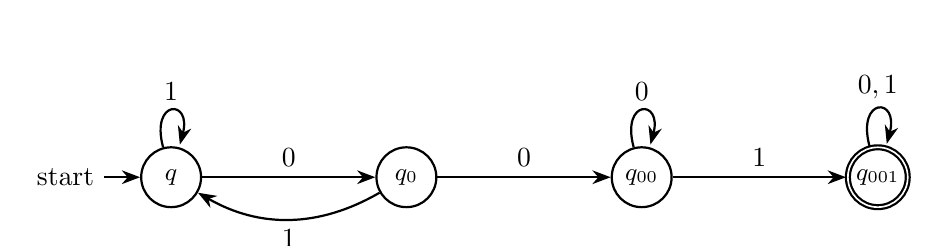
\begin{tikzpicture}[auto,>=Stealth,thick,node distance=22mm,
  every state/.style={minimum size=7.6mm,inner sep=1pt,font=\small}]
  \node[state,initial] (q) {$q$};
  \node[state,right=of q] (q0) {$q_0$};
  \node[state,right=of q0] (q00) {$q_{00}$};
  \node[state,accepting,right=of q00] (q001) {$q_{001}$};
  \path[->]
    (q) edge[loop above] node{$1$} ()
        edge node{$0$} (q0)
    (q0) edge[bend left] node{$1$} (q)
         edge node{$0$} (q00)
    (q00) edge[loop above] node{$0$} ()
          edge node{$1$} (q001)
    (q001) edge[loop above] node{$0,1$} ();
\end{tikzpicture}
\end{center}

On a mismatch, go to the state for the longest proper prefix of the
pattern that is still a suffix. For $001$, seeing $0$ in $q_{00}$ stays
in $q_{00}$ because the last $0$ is still a prefix.

\subsubsection{Avoids a fixed substring}

Same progress states as ``contains'', but the completed-pattern state is a
rejecting sink, and every other state is accepting. Equivalently: build
the DFA for ``contains $w$'' and swap accept/non-accept
(Sipser Ex.~1.5, Thm.~idea of Ex.~1.14a).

\textbf{Book, Ex.~1.5(a).} DFA for ``contains $ab$'', then complement:
the complement DFA accepts exactly the strings with no $ab$, i.e.\
strings in $b^*a^*$.

\subsubsection{Starts with / ends with}

\begin{itemize}[nosep]
  \item \textbf{Starts with $w$:} a chain that spells $w$, then a sink
        that stays accepting; a mismatch early goes to a dead reject.
  \item \textbf{Ends with a fixed word $w$:} track the longest prefix
        of $w$ that is also a suffix of the text read so far. This is
        a DFA with at most $|w|+1$ states. The usual NFA also has
        $|w|+1$ states (guess the start of the suffix) and is not
        smaller. Do not confuse this with $C_k=\Sigma^*a\Sigma^{k-1}$,
        ``an $a$ exactly $k$ places from the right'', which does need
        $2^k$ DFA states (Problems~1.60--1.61).
\end{itemize}

Sipser Ex.~1.6(a): begins with $1$ and ends with $0$. Remember
(first symbol, last symbol), with a ``haven't seen first symbol yet''
start state.

Sipser Ex.~1.7(a): ends with $00$, asked as a $3$-state NFA, not a DFA.

\subsubsection{Exactly / at least / at most $k$ occurrences}

Count until $k$, then freeze.

\begin{itemize}[nosep]
  \item At least $k$ $a$'s: states $0,1,\dots,k$; accept $k$; $a$
        increments until $k$, then loops; other symbols stay.
  \item Exactly $k$ $a$'s: same chain, but $k$ is accept and $k+1$ is a
        dead reject.
  \item At most $k$ $a$'s: $0,\dots,k$ accepting, $k+1$ dead reject.
\end{itemize}

Sipser Ex.~1.6(b): at least three $1$s. Four states $0,1,2,3+$.

\subsubsection{Position / length conditions}

\begin{itemize}[nosep]
  \item Length at most $5$: states $0,1,2,3,4,5$ (accept) and a dead
        state for length $\ge 6$. Sipser Ex.~1.6(g).
  \item Third symbol is $0$: states ``pos~$1$'', ``pos~$2$'',
        ``pos~$\ge 3$ and third was $0$'', ``pos~$\ge 3$ and third was
        $1$'' / too short. Sipser Ex.~1.6(d).
  \item Every odd position is $1$: track whether the next position is
        odd or even; on an odd position, $0$ goes to a dead reject.
        Sipser Ex.~1.6(i).
  \item Starts with $0$ and odd length, or starts with $1$ and even
        length: remember (first bit, length parity). Ex.~1.6(e).
\end{itemize}

\subsubsection{All strings except a finite list}

Build a trie of the forbidden strings. Accept everywhere except the
nodes that spell a forbidden word, and send unused symbols into a
general accept sink. Sipser Ex.~1.6(h): all strings except $11$ and
$111$. Ex.~1.5(h): all strings except $a$ and $b$.

\subsubsection{Empty set and $\set{\eps}$}

\begin{itemize}[nosep]
  \item Empty set: one (or more) states, $F=\varnothing$. Ex.~1.6(m).
  \item All strings except $\eps$: start non-accept, every other
        reachable state accept. Ex.~1.6(n).
  \item $\set{\eps}$: start accept, every positive-length string goes
        to a dead reject. Related NFA: Ex.~1.7(g), one accept state
        with no transitions.
  \item $\set{\eps,0}$: start accept; $0$ goes to a second accept
        state whose every outgoing arrow goes to a dead reject; $1$
        goes from the start straight to the dead reject. Do not make
        the ``after $0$'' state a sink, or $00,000,\ldots$ are
        accepted. Ex.~1.6(k).
\end{itemize}

\subsubsection{Boolean combinations of finite conditions}

If the language is ``$P$ and $Q$'' or ``$P$ or $Q$'', build a DFA for
each and take the product (next type). Sipser Ex.~1.4 and 1.6(l).

\subsubsection{Modular arithmetic}

\begin{itemize}[nosep]
  \item Residue of a count modulo $n$: $n$ states. Sipser Ex.~1.13 /
        Example~1.15 style; Problem~1.36: $\{a^k\mid k\text{ is a
        multiple of }n\}$ is regular.
  \item Binary number $\equiv 0\pmod n$: states $0,1,\dots,n-1$
        storing the value of the prefix modulo $n$. Reading bit $b$
        updates $r\mapsto (2r+b)\bmod n$. Accept $0$ (decide whether
        leading zeros / $\eps$ are allowed). Problem~1.37.
  \item Running sum modulo $3$ with \texttt{RESET}: Sipser
        Example~1.13 / 1.17.
\end{itemize}

\subsubsection{Last-$k$ window}

\begin{itemize}[nosep]
  \item $C_k=\Sigma^*a\Sigma^{k-1}$: ``an $a$ exactly $k$ places from
        the right''. An NFA with $k+1$ states guesses the $a$ and then
        counts $k-1$ symbols (Problem~1.60). Any DFA needs at least
        $2^k$ states (Problem~1.61): it must remember the last $k$
        bits.
  \item $D_k=\Sigma^*a(\Sigma\cup\{\eps\})^{k-1}$: at least one $a$
        among the last $k$ symbols. A DFA with $k+1$ states remembers
        how long since the last $a$ (Problem~1.62).
\end{itemize}

\subsubsection{Comments / delimited blocks}

Sipser Ex.~1.22: strings that begin with \texttt{/\#}, end with
\texttt{\#/}, and contain no intervening \texttt{\#/}, over
$\Sigma=\{a,b,/,$\#$\}$.

States track delimiter progress: not started; saw \texttt{/}; inside
comment; inside and just saw \texttt{\#}; accepted (closed). Reject
if a close appears illegally or if the string is not exactly one
well-formed comment.

%======================================================================
\section{Product, complement, and regular operations on automata}

\subsection{Product construction: intersection or union of DFAs}
\label{type:product}

\textbf{What they can ask.}
The language is the intersection (or union) of two simpler languages.
Construct DFAs for the pieces, then combine them. Sipser Ex.~1.4;
footnote~3, p.~46.

\textbf{How to recognize it.}
The statement contains \emph{and}, \emph{or}, or is explicitly ``the
intersection of two simpler languages''.

\textbf{Method.}
Let $M_1=(Q_1,\Sigma,\delta_1,q_1,F_1)$ and
$M_2=(Q_2,\Sigma,\delta_2,q_2,F_2)$.
\begin{enumerate}
  \item States: $Q_1\times Q_2$.
  \item Start: $(q_1,q_2)$.
  \item $\delta((r,s),a)=(\delta_1(r,a),\delta_2(s,a))$.
  \item Intersection: $F=F_1\times F_2$.
  \item Union: $F=(F_1\times Q_2)\cup(Q_1\times F_2)$.
\end{enumerate}
You may then merge equivalent states if you want a smaller diagram.

\textbf{Important cases.}
\begin{itemize}[nosep]
  \item ``At least three $a$'s \emph{and} at least two $b$'s'': product
        of a $4$-state $a$-counter and a $3$-state $b$-counter.
  \item ``Even number of $a$'s \emph{and} one or two $b$'s''.
  \item ``Even length \emph{and} odd number of $a$'s''.
  \item ``Even $a$'s \emph{or} exactly two $1$s'': union product, or
        later an NFA with $\eps$-union (Ex.~1.6(l), 1.7(c)).
\end{itemize}

\textbf{Mini-example.}
Sipser Ex.~1.4(b). \textbf{Book:} DFA for exactly two $a$'s, DFA for
at least two $b$'s, then the intersection product; some states can be
merged afterwards.

\textbf{Common mistake.}
Using $F_1\times F_2$ when the question asked for union.

\subsection{Complement of a DFA}
\label{type:complement}

\textbf{What they can ask.}
The language is ``does not contain\ldots'', ``any string not in
$R$'', or ``the complement of \ldots''. Sipser Ex.~1.5, 1.14.

\textbf{Method.}
\begin{enumerate}
  \item Build a DFA $M$ for the simpler language $B$.
  \item Swap accept and non-accept states. The new DFA recognizes
        $\overline{B}$. This is Ex.~1.14(a) and proves regular
        languages are closed under complement.
\end{enumerate}

\textbf{Important cases.}
This swap \textbf{fails for NFAs}. Ex.~1.14(b): if an NFA can reject
by getting stuck, or can be in both an accept and a non-accept state,
swapping $F$ need not complement the language. Regular languages are
still closed under complement, because you first convert the NFA to a
DFA, \emph{then} swap.

\textbf{Mini-example.}
\textbf{Book, Ex.~1.5(a)--(b).} Draw the DFA for ``contains $ab$''
(resp.\ $baba$), then swap accepting status.

\textbf{Common mistake.}
Complementing an NFA by swapping $F$. Also: forgetting that the DFA
must be complete (every $(q,a)$ defined) before you swap; otherwise
missing transitions silently reject and the complement is wrong.

\subsection{NFA constructions for union, concatenation, star}
\label{type:nfa-ops}

These are Sipser Theorems~1.45, 1.47, 1.49. Exam questions say
``use the construction in the proof of Theorem~\ldots''.

\textbf{What they can ask.}
Give the state diagram of an NFA for $A\cup B$, $A\circ B$, or $A^*$,
using the official construction. Ex.~1.8, 1.9, 1.10.

\textbf{Method.}

\paragraph{Union (Thm.~1.45).}
Add a new start state $q_0$ with $\eps$-arrows to the two old start
states. Accept states $=$ old accept states of both machines.

\paragraph{Concatenation (Thm.~1.47).}
Keep $N_1$'s start state. From every accept state of $N_1$, add an
$\eps$-arrow to $N_2$'s start. Accept states $=$ accept states of
$N_2$ only.

\paragraph{Star (Thm.~1.49).}
Add a \emph{new} start state $q_0$ that is also accepting, with an
$\eps$-arrow to the old start. From every old accept state, add an
$\eps$-arrow back to the old start. The accept set is
$F=\{q_0\}\cup F_1$: every old accept state remains accepting, and
the new start is accepting as well (so $\eps\in A^*$). Do
\textbf{not} merely mark the old start accepting.

\textbf{Why a new start state is required.}
Ex.~1.15: if you only add $\eps$-loops from old accepts to the old
start and mark the old start accepting, you may accept strings that
are not in $A^*$. The new start state accepts $\eps$ without
accidentally accepting a nonempty prefix that happens to leave you in
the old start.

\textbf{Common mistake.}
For star, making the original start state accepting. Sipser explicitly
warns that this ``slightly bad idea'' adds extra strings.

\subsection{Single-accept-state NFA}

\textbf{What they can ask.}
Prove every NFA has an equivalent NFA with one accept state.
Ex.~1.11.

\textbf{Method (Book).}
Keep the old machine. Add a new state $q_{\mathrm{accept}}$ with no
outgoing transitions. From every old accept state add an $\eps$-arrow
to $q_{\mathrm{accept}}$. The only accept state is
$q_{\mathrm{accept}}$.

%======================================================================
\section{Constructing an NFA (when a DFA is the wrong tool)}
\label{type:nfa-design}

\textbf{What they can ask.}
Give an NFA with a specified (usually small) number of states.
Ex.~1.7.

\textbf{How to recognize it.}
The question mentions an NFA, or a state bound that is smaller than
any DFA, or the language is a regular expression / ``ends with $w$'' /
union of simple pieces.

\textbf{Method.}
Use nondeterminism to \emph{guess} a position or a branch.
\begin{itemize}[nosep]
  \item Ends with $w$: stay in a start loop on $\Sigma$, then
        nondeterministically jump into a chain that spells $w$.
  \item Language given by a regex: build the regex-NFA
        (Section~\ref{type:re-nfa}).
  \item Union: $\eps$-branch (Thm.~1.45).
  \item ``$0$'' as a language: two states, one $0$-arrow, no extra
        symbols. Ex.~1.7(d).
  \item $0^*1^*0^+$: three-state chain with loops. Ex.~1.7(e).
  \item $1^*(001^+)^*$: loop on $1$ at start, then a $001^+$ gadget
        that returns. Ex.~1.7(f), Book has the diagram.
\end{itemize}

\textbf{Mini-example.}
Ex.~1.7(a): ends with $00$, three states. \textbf{Constructed here}
(the Book diagram may differ). Start loops on $0,1$;
nondeterministically take $0$ into a ``just saw $0$'' state, then
another $0$ into an accept; from accept, $0$ may stay (the last two
symbols are still $00$) and $1$ returns to start.

\textbf{Common mistake.}
Building a full DFA when the question demanded an NFA with $k$
states. A DFA for one fixed suffix $w$ needs only about $|w|+1$
states. The exponential blow-up is for $C_k$ (the $k$-th symbol
from the right is $a$), not for a fixed pattern.

%======================================================================
\section{NFA to DFA: subset construction}
\label{type:subset}

\textbf{What they can ask.}
Convert this NFA to an equivalent DFA. Ex.~1.16, 1.17; Thm.~1.39;
Example~1.41.

\textbf{How to recognize it.}
``Convert the NFA'', ``equivalent DFA'', ``subset construction'',
``only the reachable part''.

\textbf{Method (Sipser Thm.~1.39).}
Let $N=(Q,\Sigma,\delta,q_0,F)$.
\begin{enumerate}
  \item For $R\subseteq Q$ define the $\eps$-closure
        \[
          E(R)=\{\,q\mid q\text{ is reachable from $R$ by $0$ or more
          $\eps$-arrows}\,\}.
        \]
  \item DFA states: $\powerset{Q}$ (in practice, only reachable
        subsets).
  \item Start state: $E(\{q_0\})$.
  \item $\displaystyle\delta'(R,a)=E\Bigl(\bigcup_{r\in R}\delta(r,a)\Bigr)$.
        Follow $a$-arrows from every state in $R$, then take
        $\eps$-closure.
  \item Accept: every subset that intersects $F$.
  \item Begin at the start subset and add only subsets you actually
        reach. Drop unreachable subsets (Sipser does this in
        Example~1.41).
\end{enumerate}

\textbf{Important cases.}
\begin{itemize}[nosep]
  \item No $\eps$-arrows: $E(R)=R$, start is $\{q_0\}$.
  \item $\varnothing$ is a legal DFA state (the ``dead'' set). It
        loops to itself on every symbol.
  \item An $n$-state NFA yields at most $2^n$ DFA states. This bound
        is tight in general (Problems~1.60--1.61, 1.69).
\end{itemize}

\textbf{Mini-example.}
Example~1.41 / $N_4$ with states $\{1,2,3\}$. Start is $E(\{1\})=\{1,3\}$.
Accepting subsets are those containing $1$. After removing unreachable
$\{1\}$ and $\{1,2\}$, a $6$-state DFA remains.

\textbf{Common mistake.}
Forgetting $\eps$-closure on the start state or after each symbol.
Sipser follows $\eps$-arrows \emph{after} reading the symbol.

%======================================================================
\section{Regular expressions}

\subsection{Write a regular expression for a language}
\label{type:write-re}

\textbf{What they can ask.}
Give a regular expression generating the language of Ex.~1.6, or a
language described in English. Ex.~1.18, 1.12, 1.22(b).

\textbf{How to recognize it.}
``Give a regular expression'', ``generate'', no automaton required.

\textbf{Method: pattern catalogue.}
Let $\Sigma$ be the alphabet.
\begin{center}
\begin{tabular}{@{}ll@{}}
\toprule
English condition & Typical regex \\
\midrule
anything & $\Sigma^*$ \\
contains $w$ & $\Sigma^*w\Sigma^*$ \\
starts with $w$ & $w\Sigma^*$ \\
ends with $w$ & $\Sigma^*w$ \\
does not contain $ab$ & $b^*a^*$ \\
$a^*b^*$ & $a^*b^*$ \\
even number of $a$'s (over $\{a,b\}$) & $b^*(ab^*ab^*)^*$ \\
exactly two $a$'s & $b^*ab^*ab^*$ \\
at least three $1$s & $\Sigma^*1\Sigma^*1\Sigma^*1\Sigma^*$ \\
length at most $5$ & $\eps\cup\Sigma\cup\cdots\cup\Sigma^5$ \\
$(aaa)^*$ & strings of $a$'s whose length is a multiple of $3$ \\
empty set & $\varnothing$ \\
only $\eps$ & $\eps$ \\
all except $\eps$ & $\Sigma\Sigma^*$ or $\Sigma^+$ \\
\bottomrule
\end{tabular}
\end{center}

For a Boolean combination: use $\cup$ (union), concatenation, and
complement-via-DFA if needed. If the language is easier as a DFA,
build the DFA and convert by the GNFA method
(Section~\ref{type:gnfa}).

\textbf{Mini-example.}
Ex.~1.12: even number of $a$'s, odd number of $b$'s, and no substring
$ab$. \textbf{Constructed here.} No $ab$ means all $b$'s come first, so
the language sits inside $b^*a^*$. Odd $b$'s then even $a$'s:
$(bb)^*b(aa)^*$.

\textbf{Common mistake.}
Writing $\Sigma^*-\{11,111\}$ as if set-difference were a regex
operator. Regex has only $\cup$, concat, and star. Encode exceptions
by listing the allowed strings, or convert a DFA.

\subsection{Membership in a regular expression}
\label{type:re-member}

\textbf{What they can ask.}
Give two strings in the language and two not in it. Ex.~1.20.

\textbf{Method.}
Expand the expression into the strings it can generate.
\begin{itemize}[nosep]
  \item $a^*b^*$: $aaabb$ yes; $ba$ no.
  \item $a(ba)^*b$: starts with $a$, ends with $b$, strictly
        alternating. $ab$ yes; $a$ no.
  \item $a^*\cup b^*$: no mixing. $aaa$ yes; $ab$ no.
  \item $(aaa)^*$: $\eps,aaa,aaaaaa$; $aa$ no.
  \item $\Sigma^*a\Sigma^*b\Sigma^*a\Sigma^*$: at least two $a$'s with
        a $b$ somewhere between them.
  \item $(a\cup ba\cup bb)\Sigma^*=\Sigma^*\setminus\{\eps,b\}$:
        everything except $\eps$ and the single symbol $b$.
\end{itemize}

\subsection{Regular expression $\to$ NFA}
\label{type:re-nfa}

\textbf{What they can ask.}
Convert the regex to an NFA by Lemma~1.55 / Thm.~1.54. Ex.~1.19,
1.28.

\textbf{How to recognize it.}
``Use the procedure described in Lemma~1.55'' or ``Theorem~1.54''.
Then you must use Sipser's inductive gadgets, not a clever minimal
NFA.

\textbf{Method (Sipser).}
Recurse on the expression.
\begin{enumerate}
  \item Symbol $a$: two states, one $a$-arrow from start to accept.
  \item $\eps$: one accept state, no transitions.
  \item $\varnothing$: one non-accept state, no transitions.
  \item $R_1\cup R_2$: build both NFAs, apply Thm.~1.45.
  \item $R_1\circ R_2$: build both, apply Thm.~1.47.
  \item $R_1^*$: build $N_1$, apply Thm.~1.49 (new start/accept).
\end{enumerate}

\textbf{Mini-example.}
Example~1.56: $(ab\cup a)^*$ is built from $a$, then $ab$, then
union, then star. The procedure produced $8$ states; a $2$-state NFA
also exists, but that is not what the procedure asks for.

\textbf{Common mistake.}
Simplifying mid-construction when the question said ``use the
procedure''. Also: $\varnothing^*$ is $\{\eps\}$, not $\varnothing$.
Ex.~1.19(c).

\subsection{DFA/NFA $\to$ regular expression via GNFA}
\label{type:gnfa}

\textbf{What they can ask.}
Convert the automaton to a regex by Lemma~1.60. Ex.~1.21;
Examples~1.66 and 1.68.

\textbf{Method (Sipser CONVERT).}
\begin{enumerate}
  \item Convert the DFA to a GNFA in special form:
        \begin{itemize}[nosep]
          \item add a new start state with an $\eps$-arrow to the old
                start;
          \item add a new accept state with $\eps$-arrows from all old
                accepts;
          \item the new start has no incoming arrows; the new accept
                has no outgoing arrows;
          \item except for those, every pair of states (including
                self-loops) has exactly one arrow, labelled by a regex
                (use $\varnothing$ if there was no transition; union
                labels if several symbols went the same way).
        \end{itemize}
  \item While more than $2$ states remain, rip an old state
        $q_{\mathrm{rip}}$. For every remaining pair $(q_i,q_j)$ replace
        the label $R_4$ from $q_i$ to $q_j$ by
        \[
          (R_1)(R_2)^*(R_3)\;\cup\; R_4,
        \]
        where $R_1$ is $q_i\to q_{\mathrm{rip}}$, $R_2$ is the loop
        $q_{\mathrm{rip}}\to q_{\mathrm{rip}}$, $R_3$ is
        $q_{\mathrm{rip}}\to q_j$.
  \item When only start and accept remain, the unique arrow label is
        the regular expression.
\end{enumerate}

\textbf{Mini-example.}
Example~1.66: ripping state $2$ between $1$ and the new accept gives
$b(a\cup b)^*$ after simplifying
$(b)(a\cup b)^*(\eps)\cup\varnothing$.

\textbf{Common mistake.}
Forgetting the old direct arrow $R_4$ in the union. Forgetting
self-loops on $q_{\mathrm{rip}}$. Drawing $\varnothing$-arrows and then
dropping them from the algebra incorrectly
($R\cup\varnothing=R$, but $R\varnothing=\varnothing$).

%======================================================================
\section{Proving a language is regular}
\label{type:show-regular}

Not every regularity proof is ``draw a DFA''. Sipser's Problems use
several other patterns.

\subsection{Closure-construction proofs}

\textbf{What they can ask.}
Show the class of regular languages is closed under reverse, shuffle,
homomorphism, $\mathrm{NOPREFIX}$, $\mathrm{DROP\text{-}OUT}$,
quotient, \ldots\ Ex./Problems~1.31, 1.40--1.45, 1.66--1.68, 1.70.

\textbf{How to recognize it.}
An operation on languages is defined, and you must show ``if $A$ is
regular then the result is regular''.

\textbf{Method.}
\begin{enumerate}
  \item Start from a DFA or NFA $M$ for $A$.
  \item Describe a new automaton $M'$ whose states remember whatever
        finite information the operation needs.
  \item Argue $M'$ accepts exactly the operated language.
\end{enumerate}

\textbf{Reusable constructions.}
\begin{itemize}
  \item \textbf{Reverse $A^R$ (1.31).} Reverse all arrows, swap start
        and accept. Multiple old accepts: add a new start with
        $\eps$-arrows to all old accepts. The result is an NFA.
  \item \textbf{$\mathrm{NOPREFIX}(A)$ (1.40(a), Book).} From a DFA
        for $A$, delete every outgoing transition of an accept state
        (formally $\delta'(r,a)=\{\delta(r,a)\}$ if $r\notin F$, and
        $\varnothing$ if $r\in F$). The result is an NFA. It accepts
        $w\in A$ only if no proper prefix of $w$ was already in $A$.
  \item \textbf{$\mathrm{NOEXTEND}(A)$ (1.40(b)).} Accept states of
        $A$ from which no (positive-length) path leads to an accept
        state.
  \item \textbf{Perfect shuffle (1.41).} States
        $Q_1\times Q_2\times\{1,2\}$. The last bit is the phase:
        component~1 reads on phase~$1$, component~2 reads on
        phase~$2$, then the phase flips. Accept only in the phase
        that corresponds to even length, with both component states
        accepting. A plain $Q_1\times Q_2$ product is not enough,
        because it does not remember whose turn it is.
  \item \textbf{Shuffle (1.42).} Product; at each step
        nondeterministically feed the symbol to either component.
  \item \textbf{$\mathrm{DROP\text{-}OUT}(A)$ (1.43).} From a DFA
        $M$ for $A$, build an NFA that simulates $M$ but omits exactly
        one symbol of the original word. States $Q\times\{0,1\}$; the
        bit records whether the deletion has already happened.
        Ordinary $a$-transitions keep the bit and follow $\delta$.
        For every $q$ and $a\in\Sigma$ add an $\eps$-move
        $(q,0)\xrightarrow{\eps}(\delta(q,a),1)$: take the old
        $a$-transition without reading a new input symbol. Start
        $(q_0,0)$; accept $F\times\{1\}$. This forces exactly one
        deletion.
  \item \textbf{$B\mathbin{\leftarrow^1}C$ (1.44, Book).} Product
        NFA $Q_B\times Q_C$. On $0$, only $M_B$ moves; on $1$, both
        move; on $\eps$, only $M_C$ may consume a $0$ (guess extra
        $0$s in the hidden string $y$). Accept $F_B\times F_C$. This
        checks $w\in B$ and guesses some $y\in C$ with the same
        number of $1$s.
  \item \textbf{Quotient $A/B=\{w\mid wx\in A\text{ for some }x\in B\}$
        (1.45).} If $A$ is regular, $B$ arbitrary: from the DFA for
        $A$, a state $q$ is accepting in the new machine iff some
        string of $B$ takes $q$ to an old accept state. You do
        \emph{not} need $B$ to be regular to define $F'$, but
        computing $F'$ may be non-constructive if $B$ is arbitrary.
  \item \textbf{Homomorphism (1.66).} Replace each $a$-arrow by a
        path spelling $f(a)$. The result may be an NFA, not a DFA.
  \item \textbf{Rotational closure $RC(A)=\{yx\mid xy\in A\}$ (1.67).}
        Guess the rotation point: jump into the middle of $M$, finish,
        then from start run the skipped prefix.
  \item \textbf{$A$ avoids $B$ (1.70).} Intersect $A$ with the
        complement of $\Sigma^*B\Sigma^*$ (the latter is regular if
        $B$ is).
  \item \textbf{First halves $A_{1/2}$ (1.57).} A DFA for $A$ can
        be converted to one that accepts $x$ iff some $y$ of equal
        length takes the state after $x$ to an accept state
        (product of the forward machine with a reverse-subset
        tracker). Regular languages are closed under this.
\end{itemize}

\subsection{``Looks nonregular, but is regular''}

Sipser warns (p.~77) that intuition about ``needing to count'' is
unreliable.

\textbf{What they can ask.}
Show $D$ is regular, even though it mentions equality of counts.
Problems~1.48, 1.49(a), 1.71(a).

\textbf{Method.}
Rewrite the language so a finite-memory DFA becomes obvious.

\begin{itemize}
  \item \textbf{Equal number of substrings $01$ and $10$
        (Problem~1.48).} \textbf{Constructed here.} A string over
        $\{0,1\}$ alternates blocks. The two patterns count the
        number of switches. They differ by at most $1$, and they are
        equal iff the string starts and ends with the same symbol
        (or is unary). That is regular.
  \item \textbf{$B=\{1^ky\mid y\text{ contains at least }k\text{ ones}\}$
        (1.49(a)).} \textbf{Constructed here.} Once $k\ge 1$, this is
        just ``starts with $1$ and contains at least two $1$s''.
        Regular.
  \item \textbf{$A=\{0^ku0^k\mid k\ge 1,\,u\in\Sigma^*\}$ (1.71(a)).}
        \textbf{Constructed here.} Any string of length at least $2$
        that starts and ends with $0$ can be written this way with
        $k=1$. So $A=0\Sigma^*0$, which is regular.
  \item \textbf{Column languages that add binary numbers
        (1.32--1.34).} Process columns from the \emph{right} (use
        reverse, 1.31). States store the carry. Regular. Comparing
        two rows (1.34) is a left-to-right carry/``greater already''
        bit.
\end{itemize}

\textbf{Common mistake.}
Applying the pumping lemma to a language that is actually regular
(Ex.~1.30 does this to $0^*1^*$). If a simple DFA exists, pumping
cannot succeed.

\subsection{Algebraic identities}

Ex.~1.23: $B=B^+$ iff $BB\subseteq B$. \textbf{Book:} one direction
is $BB\subseteq B^+\subseteq B$ if $B=B^+$; the other is induction
on the number of concatenated factors.

%======================================================================
\section{The pumping lemma for regular languages}
\label{type:pump-reg}

This is the most examined nonregularity tool in Chapter~1
(Thm.~1.70, Examples~1.73--1.77, Ex.~1.29, Problems~1.46, 1.47,
1.53--1.55).

\subsection{When to use it}

Use the pumping lemma when the question is
\begin{itemize}[nosep]
  \item ``show $L$ is not regular'', or
  \item ``show $L$ is not regular using the pumping lemma''.
\end{itemize}
Do \emph{not} use it to prove regularity. Do not use it as the first
tool if a closure argument is shorter (equal counts
$\cap\,0^*1^*=\{0^n1^n\}$).

If the language is regular, the lemma cannot yield a contradiction.
If a language ``acts regular'' in the pumping lemma but is still
nonregular, that is Problem~1.54: the lemma is necessary, not
sufficient.

\subsection{The exam recipe}

Assume $L$ is regular. Let $p$ be the pumping length given by the
lemma. You must produce one string $s\in L$ with $|s|\ge p$ that
\textbf{cannot be pumped}.

The structural conditions on a candidate split $s=xyz$ are only
\begin{enumerate}[nosep]
  \item $|y|>0$,
  \item $|xy|\le p$.
\end{enumerate}
You do not choose $x,y,z$. For every split that satisfies those two
conditions, you must find some $i\ge 0$ with $xy^iz\notin L$.
(Condition~1 of the lemma, ``$xy^iz\in L$ for all $i$'', is what
you contradict; it is not a filter on which splits you consider.)
Condition $|xy|\le p$ is your friend: $y$ lives inside the first
$p$ symbols.

\textbf{Numbered attack.}
\begin{enumerate}
  \item Assume $L$ regular; let $p$ be the pumping length.
  \item Choose $s\in L$ with $|s|\ge p$ that encodes the
        \emph{essence} of the nonregularity (usually a long block of
        one symbol, length $p$ or $p!$ or $p^2$ or $2^p$).
  \item Consider an arbitrary split $s=xyz$ with $|y|>0$ and
        $|xy|\le p$. Use the length bound to restrict what $y$
        can be.
  \item Pick a single $i$ (often $i=2$ or $i=0$) that breaks
        membership for that split. If several geometrically different
        splits remain possible, case-split on them.
  \item Conclude $s$ cannot be pumped, contradiction.
\end{enumerate}

\subsection{How to choose $s$}

\begin{center}
\begin{tabular}{@{}llp{6.6cm}@{}}
\toprule
Language & Good $s$ & Why \\
\midrule
$\{0^n1^n\}$ & $0^p1^p$ & $|xy|\le p$ forces $y$ to be only $0$s \\
equal $\#$ of $0$s and $1$s & $0^p1^p$, not $(01)^p$ &
$(01)^p$ \emph{can} be pumped \\
$\{ww\}$ & $0^p10^p1$, not $0^p0^p$ & $0^{2p}$ can be pumped \\
$\{0^n1^n2^n\}$ & $0^p1^p2^p$ & cases: $y$ monochrome or mixed \\
$\{1^{n^2}\}$ & $1^{p^2}$ & pump up lands between squares \\
$\{a^{2^n}\}$ & $a^{2^p}$ & $|xyyz|$ is strictly between $2^p$ and
$2^{p+1}$ \\
$\{0^i1^j\mid i>j\}$ & $0^{p+1}1^p$ & pump \emph{down} ($i=0$) \\
$\{0^m1^n\mid m\neq n\}$ & $0^p1^{p+p!}$ & pump $p!/|y|$ times \\
\bottomrule
\end{tabular}
\end{center}

\subsection{How to choose $i$}

\begin{itemize}[nosep]
  \item \textbf{Pump up, $i=2$:} default. Breaks equalities
        $n=n$, order, or ``length is a square / power of two''.
  \item \textbf{Pump down, $i=0$:} when the language is an inequality
        such as more $0$s than $1$s (Example~1.77). Pumping up stays
        in the language.
  \item \textbf{Pump a designed number of times:} for
        $\{0^m1^n\mid m\neq n\}$, Book 1.46(b) uses
        $s=0^p1^{p+p!}$ and $i=1+p!/|y|$, so the $0$-count becomes
        $p+p!$ and equals the $1$-count.
\end{itemize}

\subsection{Typical case splits}

When $s=0^p1^p$ and you do \emph{not} invoke condition~3:
\begin{enumerate}[nosep]
  \item $y$ is only $0$s $\Rightarrow$ $xyyz$ has more $0$s than $1$s;
  \item $y$ is only $1$s $\Rightarrow$ more $1$s than $0$s;
  \item $y$ straddles the boundary $\Rightarrow$ symbols out of order.
\end{enumerate}
Sipser notes that condition~3 kills cases 2 and 3 immediately
(Example~1.73). Prefer invoking $|xy|\le p$.

When $s=0^p1^p2^p$ (Book 1.29(a)):
\begin{enumerate}[nosep]
  \item $y$ monochrome $\Rightarrow$ the three counts become unequal;
  \item $y$ mixed $\Rightarrow$ the symbols are out of order.
\end{enumerate}

\subsection{Worked patterns from the book}

\paragraph{$\{0^n1^n\}$ (Example~1.73).}
$s=0^p1^p$. Condition~3 $\Rightarrow$ $y\in 0^+$. Then $xyyz$ has
more $0$s than $1$s.

\paragraph{Equal number of $0$s and $1$s (Example~1.74).}
Same $s=0^p1^p$. Without condition~3 you could take $y=0^p1^p$ and
pump forever. With it, $y$ is only $0$s. Alternative (often cleaner):
if this language $C$ were regular then
$C\cap 0^*1^*=\{0^n1^n\}$ would be regular.

\paragraph{$\{ww\}$ (Example~1.75).}
$s=0^p10^p1$. Condition~3 $\Rightarrow$ $y$ is in the first block of
$0$s, so $xyyz$ is not $ww$. Bad choice: $0^{2p}$, which pumps.

\paragraph{Unary squares (Example~1.76).}
$D=\{1^{n^2}\}$, $s=1^{p^2}$. Then
$p^2<|xyyz|\le p^2+p<(p+1)^2$, so the length is not a square.

\paragraph{Unary powers of two (Book 1.29(c)).}
$s=a^{2^p}$. Then $2^p<|xyyz|<2^{p+1}$.

\paragraph{More $0$s than $1$s (Example~1.77).}
$s=0^{p+1}1^p$. Pumping up stays in the language. Pump down:
$xz$ does not have more $0$s than $1$s.

\paragraph{$\{0^m1^n\mid m\neq n\}$ (Book 1.46(b)).}
Closure way: complement intersect $0^*1^*$ is $\{0^k1^k\}$. Direct
pumping way: $s=0^p1^{p+p!}$, pump $p!/|y|$ extra copies of $y$.

\paragraph{Not a palindrome (1.46(c)).}
\textbf{Constructed here.} Complement is the palindromes, which is
nonregular, but regular languages \emph{are} closed under complement,
so if ``not a palindrome'' were regular then palindromes would be
too. To pump directly is messier; prefer closure.

\paragraph{$\{wtw\mid w,t\in\{0,1\}^+\}$ (1.46(d)).}
\textbf{Constructed here.} Intersect with the regular language
$0^+10^+1$ to get $\{0^n10^n1\mid n\ge 1\}$, which is nonregular
by the same argument as $\{ww\}$.

\paragraph{$Y$ with distinct $1$-blocks (1.47).}
\textbf{Constructed here.} Take
$s=1^p\#1^{p-1}\#\cdots\#1\#$. Condition~$3$ puts $y$ inside the
first block. Pump \emph{down} ($i=0$): the first block becomes
shorter than $p$ and duplicates a later block length. Pumping up
would make it longer than every later block and would not give a
contradiction.

\paragraph{$\mathrm{ADD}=\{x{=}y{+}z\}$ in binary (1.53).}
\textbf{Constructed here.} Intersect with the regular language
$1^*{=}0^*{+}1^*$ to force strings of the form $1^n{=}0^m{+}1^n$,
then pump as for $\{0^n1^n\}$.

\subsection{Common traps}

\begin{enumerate}
  \item \textbf{Bad $s$.} $(01)^p$ for equal counts; $0^{2p}$ for
        $\{ww\}$; $0^p1^p$ for $0^*1^*$ (Ex.~1.30). The string must
        be in $L$ \emph{and} unpumpable under every legal split.
  \item \textbf{Choosing the split yourself} and only checking that
        one split. You must beat \emph{all} splits with $|y|>0$ and
        $|xy|\le p$.
  \item \textbf{Forgetting $i=0$.} Some languages are closed under
        pumping up.
  \item \textbf{Pumping lemma does not characterize regular languages.}
        Problem~1.54: $F=\{a^ib^jc^k\mid\text{if }i=1\text{ then }j=k\}$
        is nonregular, yet it satisfies the three pumping conditions
        for $p=2$ (pump inside a long $a$-block, or avoid the $i=1$
        slice). There is no contradiction with the lemma because the
        lemma never claimed the converse.
  \item \textbf{Ex.~1.30 error.} $0^*1^*$ \emph{is} regular. The fake
        proof chose $s=0^p1^p$ and quoted Example~1.73, but
        Example~1.73 shows $s$ cannot be pumped \emph{while staying
        in $\{0^n1^n\}$}, not while staying in $0^*1^*$. In $0^*1^*$,
        $s$ pumps easily.
\end{enumerate}

\subsection{Minimum pumping length}
\label{type:min-pump}

\textbf{What they can ask.}
Give the minimum pumping length of a given regular language, with
justification. Problem~1.55.

\textbf{Method.}
The minimum pumping length is the smallest $p$ such that every
string in $A$ of length $\ge p$ can be pumped. A candidate $p$
fails if \emph{any} unpumpable member has length at least $p$, not
necessarily length exactly $p-1$. If $U$ is the (finite, for a
regular language with a pumping length) set of unpumpable members
of $A$ and $U\neq\varnothing$, then
\[
  p_{\min}=1+\max\{\,|s|:s\in U\,\}.
\]
If $U=\varnothing$ (every string in $A$ pumps, including $\eps$),
then $p_{\min}=0$. Sipser's selected solution to 1.55(b) treats
$p=0$ as a legal candidate and rejects it because $\eps$ cannot be
pumped.

\begin{enumerate}
  \item List the unpumpable strings in $A$ (usually a few short
        ones). Let $p$ be one more than the longest of them.
  \item For every $s\in A$ with $|s|\ge p$, exhibit a split with
        $|y|>0$ and $|xy|\le p$ that stays in $A$ when pumped.
\end{enumerate}

\textbf{Values.}
\begin{itemize}[nosep]
  \item $0001^*$: $p=4$ because $000$ cannot be pumped.
        \textbf{Book} (1.55(a)).
  \item $0^*1^*$: $p=1$ ($\eps$ cannot be pumped; every nonempty
        string can). \textbf{Book} (1.55(b)).
  \item $0^*1^+0^+1^*\cup 10^*1$: $p=3$ ($11$ cannot be pumped).
        \textbf{Book} (1.55(d)).
  \item $\{\eps\}$: $p=1$. \textbf{Constructed here} (1.55(f) has
        no selected solution). $\eps$ is unpumpable, and there is
        no longer string, so every $p\ge 1$ works and $1$ is
        smallest among those if $p=0$ is rejected for the same
        reason as in 1.55(b).
  \item $\Sigma^*$: $p=1$. \textbf{Constructed here.} $\eps$ is
        unpumpable; every nonempty string pumps as $x=\eps$,
        $y=$ first symbol.
  \item Finite language whose longest word has length $n$:
        $p=n+1$. \textbf{Constructed here.} A longest word cannot
        be pumped, and every string of length $\ge n+1$ is absent,
        so the claim is vacuous. Hence $1011$ has minimum pumping
        length $5$.
\end{itemize}

%======================================================================
\section{Myhill--Nerode, distinguishability, and state lower bounds}
\label{type:mn}

\textbf{What they can ask.}
\begin{itemize}[nosep]
  \item Show $x\equiv_L y$ is an equivalence relation (1.51).
  \item State and use the Myhill--Nerode theorem (1.52).
  \item Prove no DFA with fewer than $k$ states recognizes $L$
        (1.39, 1.61, 1.69).
\end{itemize}

\textbf{How to recognize it.}
Words: distinguishable, pairwise distinguishable, index, smallest
DFA, ``no DFA with fewer than $k$ states''.

\textbf{Method.}
Strings $x,y$ are \textbf{distinguishable by $L$} if some $z$ has
exactly one of $xz,yz$ in $L$.

\begin{enumerate}
  \item To prove a DFA lower bound of $k$: exhibit $k$ strings that
        are pairwise distinguishable by $L$. By 1.52(a), any DFA needs
        at least $k$ states (pigeonhole: two of them land in the same
        state, then no $z$ can distinguish them).
  \item Myhill--Nerode (Book 1.52): $L$ is regular iff it has finite
        index, and the index equals the number of states of the
        minimal DFA.
\end{enumerate}

\textbf{Mini-examples.}
\begin{itemize}[nosep]
  \item $C_k=\Sigma^*a\Sigma^{k-1}$: the $2^k$ distinct strings of
        length $k$ are pairwise distinguishable (the distinguishing
        continuation is a suitable suffix of length $0$ to $k-1$).
        Problem~1.61.
  \item $WW_k=\{ww\mid |w|=k\}$: the $2^k$ strings of length $k$ are
        pairwise distinguishable by appending the matching $w$.
        Problem~1.69.
  \item For each $k>1$ there is a language needing exactly $k$ DFA
        states (1.39): e.g.\ $\{w\mid |w|\equiv 0\pmod k\}$.
\end{itemize}

\textbf{Common mistake.}
Giving $k$ strings that are distinguishable from $\eps$ but not from
each other. Pairwise is required.

%======================================================================
\section{Finite-state transducers and odd models}

\subsection{FST: trace, define, construct}

\textbf{What they can ask.}
On this input, what states does $T$ enter and what does it output?
Give a formal definition. Draw an FST with a specified input/output
behaviour. Prove no FST can compute $w\mapsto w^R$. Ex.~1.24--1.27,
1.50.

\textbf{Method.}
An FST is a $5$-tuple $(Q,\Sigma,\Gamma,\delta,q_0)$ with
$\delta:Q\times\Sigma\to Q\times\Gamma$ (Ex.~1.25). No accept
states. Each input symbol produces exactly one output symbol.

\begin{itemize}[nosep]
  \item Trace as a DFA, but record the output label of every
        transition.
  \item Ex.~1.27: invert odd positions, copy even positions. Two
        states (odd/even position); on odd, swap $0\leftrightarrow 1$.
  \item Ex.~1.50 \textbf{Book:} no FST computes reverse. On inputs
        $00$ and $01$ the first output bits must already differ, but
        the first input bit is the same, and the FST emits the first
        output before seeing the second input.
\end{itemize}

\subsection{all-NFA}

Problem~1.38: an all-NFA accepts iff \emph{every} possible state
after reading $x$ is accepting. These still recognize exactly the
regular languages: convert to a DFA by the subset construction, and
accept a subset $R$ iff $R\subseteq F$. Include $R=\varnothing$:
the universal condition holds vacuously, so the empty set of
possible states is accepting.

\subsection{Emptiness / finiteness bounds}

Problem~1.64: an $n$-state NFA, if its language is nonempty, accepts
some string of length $\le n$ (a simple path to an accept state).
The complement, if nonempty, has a string of length $\le 2^n$
(look at the equivalent DFA). Problem~1.72: analogous bounds for
union of two DFAs.

%======================================================================
\part{Chapter 2: Context-free languages}
%======================================================================

\section{Reading a CFG}
\label{type:cfg-read}

\textbf{What they can ask.}
Variables, terminals, start variable; three strings in / not in
$L(G)$; true/false of $A\Rightarrow w$ or $A\Rightarrow^* w$;
describe $L(G)$ in English. Ex.~2.3, 2.13.

\textbf{Method.}
\begin{itemize}[nosep]
  \item Variables $V$: left-hand sides. Terminals $\Sigma$: alphabet
        symbols. Start: the specified start variable (often the first
        left-hand side).
  \item $A\Rightarrow w$ means one rule application. $A\Rightarrow^* w$
        means zero or more.
  \item To describe $L(G)$: see what recursive structure the rules
        force (matched pairs, odd length, non-palindromes, \ldots).
\end{itemize}

\textbf{Mini-example.}
Ex.~2.3. \textbf{Book:} $V=\{R,X,S,T\}$, $\Sigma=\{a,b\}$, start
$R$; $L(G)$ is all strings over $\{a,b\}$ that are \emph{not}
palindromes. $T\Rightarrow aba$ is false (one step), but
$T\Rightarrow^* aba$ is true.

\textbf{Common mistake.}
Confusing $\Rightarrow$ with $\Rightarrow^*$. Also: $\eps$ is a
palindrome, so it is \emph{not} in that $L(G)$.

\section{Derivations, parse trees, and ambiguity}
\label{type:derive}

\subsection{Give a derivation or parse tree}

\textbf{What they can ask.}
Give parse trees and (leftmost) derivations for listed strings.
Ex.~2.1, 2.8.

\textbf{Method.}
\begin{enumerate}
  \item Start from $S$.
  \item A \textbf{leftmost} derivation always replaces the leftmost
        remaining variable (Def.~2.7).
  \item The parse tree: root $S$, each internal node a variable, its
        children the right-hand side of the rule used.
  \item Yield of the tree $=$ the derived string.
\end{enumerate}

\textbf{Mini-example.}
Grammar $G_4$: $E\to E+T\mid T$, $T\to T\times F\mid F$,
$F\to(E)\mid a$. Strings $a$, $a+a$, $a+a+a$, $((a))$. Each has a
unique parse tree in $G_4$ because the grammar encodes precedence.

\subsection{Show a grammar is ambiguous}

\textbf{What they can ask.}
Show $G$ is ambiguous; give two leftmost derivations or two parse
trees for one string. Ex.~2.8, 2.9, 2.27, 2.46.

\textbf{How to recognize it.}
``Show ambiguous'', ``two different meanings'', ``two leftmost
derivations''.

\textbf{Method.}
Find one string with two different parse trees, or equivalently two
different leftmost derivations (Def.~2.7). Two derivations that only
differ in the \emph{order} of replacing unrelated variables do
\textbf{not} count---that is why Sipser uses leftmost.

\textbf{Important cases.}
\begin{itemize}
  \item \textbf{Precedence-free expressions} (grammar $G_5$ vs $G_4$,
        p.~107--108): $E\to E+E\mid E\times E\mid(E)\mid a$ derives
        $a+a\times a$ in two ways. Fix: layered variables $E$, $T$,
        $F$ as in $G_4$.
  \item \textbf{English / dangling else} (Ex.~2.8, Problem~2.27):
        ``the girl touches the boy with the flower'' --- flower
        modifies the touching vs.\ the boy. Programming:
        $\mathtt{if}$--$\mathtt{then}$--$\mathtt{else}$ dangling else.
        \textbf{Book 2.8} gives both leftmost derivations.
        Fix for 2.27: force $\mathtt{else}$ to bind to the nearest
        unmatched $\mathtt{then}$ (standard matched/unmatched
        statement grammar).
  \item \textbf{$S\to SS\mid T$, $T\to aTb\mid ab$} (2.46):
        concatenation of several $a^nb^n$ blocks can be associated
        left or right. Unambiguous repair: $S\to TS\mid T$ (always
        peel one block from the left).
\end{itemize}

\subsection{Inherently ambiguous languages}

\textbf{What they can ask.}
Is your grammar ambiguous? Why? Show the \emph{language} is
inherently ambiguous. Ex.~2.9, Problem~2.29.

\textbf{Method.}
A language is inherently ambiguous if \emph{every} CFG for it is
ambiguous (p.~108). The standard example is
\[
  A=\{a^ib^jc^k\mid i=j\text{ or }j=k\}
\]
(Problem~2.29). Showing that one union grammar derives
$a^nb^nc^n$ in two ways proves only that \emph{that grammar} is
ambiguous. That overlap is good intuition, not a proof that every
grammar is ambiguous. Sipser states the result and assigns the
proof as Problem~2.29; unless the exam asks only for the
definition and the example language, do not present the overlap
story as a complete argument.

\textbf{Common mistake.}
Proving a particular grammar is ambiguous and concluding the
language is inherently ambiguous.

\section{Constructing a CFG}
\label{type:cfg-design}

Sipser p.~106--107 gives four design techniques. Use them in
combination.

\subsection{The four Sipser techniques}

\begin{enumerate}
  \item \textbf{Union of simpler CFLs.} Build $G_i$ with start
        $S_i$, then add $S\to S_1\mid\cdots\mid S_k$.
        Example:
        $\{0^n1^n\}\cup\{1^n0^n\}$ is
        $S\to S_1\mid S_2$, $S_1\to 0S_11\mid\eps$,
        $S_2\to 1S_20\mid\eps$.
  \item \textbf{The language is regular.} Convert a DFA to a CFG:
        variable $R_i$ for state $q_i$; rule $R_i\to aR_j$ whenever
        $\delta(q_i,a)=q_j$; rule $R_i\to\eps$ if $q_i$ is accepting;
        start variable $=$ start state.
  \item \textbf{Linked / matched halves.} Use $R\to uRv$ to pair
        unbounded information on the left with corresponding
        information on the right. Prototype: $S\to 0S1\mid\eps$.
  \item \textbf{Recursive nested structure.} Put a variable in the
        place where a whole substructure may reappear (parentheses,
        expressions). Prototype: $F\to(E)\mid a$.
\end{enumerate}

\subsection{CFG pattern catalogue}

\subsubsection{Regular conditions (technique 2)}

Ex.~2.4(a), \textbf{Book:} at least three $1$s:
\[
  S\to R1R1R1R,\qquad R\to 0R\mid 1R\mid\eps.
\]
Starts and ends with the same symbol:
$S\to 0T0\mid 1T1\mid 0\mid 1$, $T\to 0T\mid 1T\mid\eps$.
Odd length: $S\to 0A\mid 1A$, $A\to 0S\mid 1S\mid\eps$.
Empty set: a start variable with no productions, or $S\to S$.

\subsubsection{$a^nb^n$ and matched pairs (technique 3)}

\begin{itemize}[nosep]
  \item $\{0^n1^n\}$: $S\to 0S1\mid\eps$.
  \item Palindromes: $S\to 0S0\mid 1S1\mid 0\mid 1\mid\eps$
        (Ex.~2.4(e)).
  \item Odd length with middle $0$ (Book 2.4(d)):
        $S\to 0\mid 0S0\mid 0S1\mid 1S0\mid 1S1$.
  \item $\{ww^R\}$: same as even-length palindromes:
        $S\to 0S0\mid 1S1\mid\eps$.
\end{itemize}

\subsubsection{Equal counts, more-of-one, Dyck-like}

\begin{itemize}
  \item Equal number of $a$'s and $b$'s (unambiguous form, 2.28(b)).
        \textbf{Constructed here.} Do \emph{not} use
        $S\to\eps\mid aSbS\mid bSaS$: it generates the language but
        is ambiguous ($abab$ has two parses). Use a first-return
        grammar, which splits uniquely at the first return of the
        $a/b$ balance to zero:
        \[
          \begin{aligned}
            S&\to\eps\mid aPbS\mid bNaS,\\
            P&\to\eps\mid aPbP,\\
            N&\to\eps\mid bNaN.
          \end{aligned}
        \]
        $P$ generates strings with $\#a=\#b$ whose every nonempty
        prefix has more $a$'s; $N$ is the symmetric $b$-first class.
  \item More $a$'s than $b$'s (Book 2.6(a)):
        $S\to TaT$, and $T$ generates at least as many $a$'s as
        $b$'s via $T\to TT\mid aTb\mid bTa\mid a\mid\eps$.
  \item Prefixes with $\#a\ge\#b$ (2.28(a)): the Dyck /
        ``never negative'' grammar, analogous to balanced parentheses
        with extra $a$'s.
\end{itemize}

\subsubsection{One equality or the other (technique 1)}

\[
  \{a^ib^jc^k\mid i=j\text{ or }j=k\}
\]
is $S\to S_1\mid S_2$ with $S_1\to AC$, $A\to aAb\mid\eps$,
$C\to cC\mid\eps$ and $S_2\to DE$, $D\to aD\mid\eps$,
$E\to bEc\mid\eps$ (Ex.~2.9). This grammar is ambiguous on
$a^nb^nc^n$. The language is inherently ambiguous (2.29).

Complement of $\{a^nb^n\}$ (2.6(b)): union of
``not of the form $a^*b^*$'' (regular) with
``$a^ib^j$ and $i\neq j$'' (two CFGs: more $a$'s, more $b$'s).

\subsubsection{A marked copy / substring on the other side}

Book 2.6(c): $\{w\#x\mid w^R\text{ is a substring of }x\}$.
\[
  S\to TX,\quad
  T\to 0T0\mid 1T1\mid \#X,\quad
  X\to 0X\mid 1X\mid\eps.
\]
$T$ guesses where the copy of $w^R$ sits after $\#$, and $X$ fills
the rest of $x$.

$\{x\#y\mid x\neq y\}$ (2.22). \textbf{Constructed here:} guess the
first position where they differ, or guess that the lengths differ.
Both are CFG-expressible (or PDA-expressible with nondeterminism).

$\{xy\mid |x|=|y|,\; x\neq y\}$ (2.23). \textbf{Constructed here:}
guess a position $i$ where the $i$th symbol of $x$ differs from the
$i$th of $y$; the CFG generates matching-length padding around that
mismatch.

\subsubsection{Twice as many / numeric relations}

$\{w\mid \#a(w)=2\cdot\#b(w)\}$ (2.21). \textbf{Constructed here:}
think of each $b$ as needing two $a$'s, placed before/after it. One
working idea is
$S\to SS\mid aSaSb\mid aSbSa\mid bSaSa\mid\eps$ plus a correctness
proof by induction (the problem asks for the proof).

$\{a^ib^j\mid i\neq j\text{ and }2i\neq j\}$ (2.24).
\textbf{Constructed here:} union of the CFLs $i>j$, $j>2i$, and
$i<j<2i$. Each inequality is CFL
($\{a^ib^j\mid j>i\}= \{a^nb^n\}b^+$, etc.).

\subsection{CFG for the complement of a simple CFL}

Problem~2.19: first describe $L(G)$ in English, then write a CFG for
the complement. This only works because that particular $L(G)$ is
simple (e.g.\ ``strings that are not of the form $a^nb^n$ plus a
regular side condition''). CFLs are \textbf{not} closed under
complement in general (Ex.~2.2).

\section{Chomsky normal form}
\label{type:cnf}

\textbf{What they can ask.}
Convert this CFG to Chomsky normal form by Thm.~2.9. Ex.~2.14;
Example~2.10. Also: a CNF derivation of a string of length $n\ge 1$
has exactly $2n-1$ steps (Problem~2.26). If a CNF grammar with $b$
variables has a derivation of $\ge 2^b$ steps, $L(G)$ is infinite
(2.35).

\textbf{How to recognize it.}
``Chomsky normal form'', ``CNF'', ``procedure of Theorem~2.9''.

\textbf{CNF restrictions (Def.~2.8).}
Every rule is $A\to BC$ or $A\to a$, and $B,C$ are not the start
variable. The only allowed $\eps$-rule is $S\to\eps$.

\textbf{Method (Sipser Thm.~2.9) --- do the stages in order.}
\begin{enumerate}
  \item \textbf{New start.} Add $S_0\to S$ so the start variable
        never appears on a right-hand side.
  \item \textbf{Eliminate $\eps$-rules} $A\to\eps$ ($A\neq S_0$).
        For every occurrence of $A$ on a right-hand side, add a
        version with that occurrence deleted. If $R\to uAvAw$, add
        $R\to uvAw$, $R\to uAvw$, and $R\to uvw$. Repeat until no
        $\eps$-rule remains except possibly $S_0\to\eps$.
  \item \textbf{Eliminate unit rules} $A\to B$. Whenever $B\to u$
        is a non-unit rule, add $A\to u$. Repeat. Do not reintroduce
        a unit rule already removed.
  \item \textbf{Binarize.} Replace $A\to u_1u_2\cdots u_k$ ($k\ge 3$)
        by $A\to u_1A_1$, $A_1\to u_2A_2$, \ldots,
        $A_{k-2}\to u_{k-1}u_k$. Replace every terminal $u_i$ that
        sits in a long or mixed rule by a new variable $U_i\to u_i$.
\end{enumerate}

\textbf{Mini-example.}
Example~2.10 starts from $S\to ASA\mid aB$, $A\to B\mid S$,
$B\to b\mid\eps$ and walks through all four stages. Ex.~2.14 is the
same procedure on $A\to BAB\mid B\mid\eps$, $B\to 00\mid\eps$.
\textbf{Constructed here} (outline): new start $S_0\to A$; remove
$B\to\eps$ and $A\to\eps$ (adding all shortened right-hand sides);
remove units $S_0\to A$, $A\to B$; replace $00$ by $U\to 0$ and
$B\to UU$; split any remaining length-${\ge}3$ right-hand sides.

\textbf{Common mistake.}
Removing $\eps$-rules but forgetting a combination of several $A$'s
on the same right-hand side. Changing the start variable without
adding a new one, then being unable to keep $S\to\eps$ when
$\eps\in L$. Applying unit elimination before $\eps$-elimination
(Sipser's order matters for the patching).

\section{CFL closure and non-closure}
\label{type:cfl-closure}

\subsection{Closed: union, concatenation, star}

Ex.~2.16. \textbf{Constructed here,} using Sipser's CFG technique~1.
If $S_1,S_2$ are the start variables (rename so variables are
disjoint):
\begin{itemize}[nosep]
  \item union: $S\to S_1\mid S_2$;
  \item concatenation: $S\to S_1S_2$;
  \item star: $S\to S_1S\mid\eps$ (or $S\to SS\mid S_1\mid\eps$).
\end{itemize}
Ex.~2.15: merely adding $S\to SS$ does \emph{not} give $A^*$, because
it may fail to add $\eps$ and, if $S$ already occurred on
right-hand sides, it can change $L(G)$. Need a fresh start variable.

Ex.~2.17: convert a regex to a CFG by the same induction as
Lemma~1.55, using the three constructions above. Hence every regular
language is a CFL.

\subsection{Closed: intersection with a regular language}

Problem~2.18(a), \textbf{Book.} Product of a PDA with a DFA: states
$Q_{\mathrm{PDA}}\times Q_{\mathrm{DFA}}$, stack unchanged, accept
$F\times F_D$. On a PDA $\eps$-move the DFA component stays put; on
a consuming move both components update. So $C\cap R$ is a CFL if
$C$ is a CFL and $R$ is regular.

\textbf{Exam use:} to prove a language $A$ is \emph{not} a CFL, pick
a regular $R$ such that $A\cap R$ is a known non-CFL
(typically $\{a^nb^nc^n\}$). Book 2.18(b):
$A=\{\text{equal numbers of }a,b,c\}$, $R=a^*b^*c^*$,
$A\cap R=\{a^nb^nc^n\}$.

\subsection{Not closed: intersection, complement, and several operations}

Ex.~2.2. $A=\{a^mb^nc^n\}$ and $B=\{a^nb^nc^m\}$ are CFLs (each
matches one pair). $A\cap B=\{a^nb^nc^n\}$ is not a CFL
(Example~2.36). By DeMorgan, CFLs are not closed under complement
either (if they were, union-of-complements would give intersection).

Also not closed, from the Problems:
perfect shuffle (2.38), shuffle (2.39), $\mathrm{NOPREFIX}$ /
$\mathrm{NOEXTEND}$ (2.41), $\mathrm{CUT}$ (2.50). They \emph{are}
closed under suffix (2.25: from a PDA, guess and skip a prefix
with $\eps$-moves / stack-neutral consumption), rotational
closure (2.49), and the quotient $A/B$ when $A$ is a CFL and $B$
is regular (2.20). If $A$ and $B$ are regular, the equal-length
concatenation $\{xy\mid x\in A,\,y\in B,\,|x|=|y|\}$ is a CFL
(2.44): a PDA runs the DFA for $A$ while pushing a counter, then
runs the DFA for $B$ while popping.

\textbf{Common mistake.}
Saying ``CFL $\cap$ CFL is a CFL''. Only CFL $\cap$ regular is
guaranteed.

\section{Constructing and tracing a PDA}
\label{type:pda}

\subsection{Design method}

\textbf{What they can ask.}
Give an informal description and/or state diagram of a PDA for a
language. Ex.~2.5, 2.7, 2.10; Examples~2.14, 2.16, 2.18.

\textbf{How to recognize it.}
``Pushdown automaton'', ``informal description of a PDA''.

\textbf{How to think (Sipser's examples).}
\begin{enumerate}
  \item What unbounded information must be matched later? That is
        what the stack stores.
  \item \textbf{Push} while reading the first region (the $0$s of
        $0^n1^n$; the $w$ of $ww^R$; the $a$'s of $a^ib^jc^k$).
  \item \textbf{Pop} while reading the matching region.
  \item Use a bottom-of-stack marker $\$$. Sipser's machines push
        $\$$ from the start state on $\eps$, and accept by seeing
        $\$$ again (empty-stack test).
  \item Acceptance is only checked at the \emph{end} of the input,
        so ``end of input'' need not be an explicit symbol.
  \item \textbf{Nondeterminism} is used to guess
        \begin{itemize}[nosep]
          \item the middle of the string ($ww^R$, palindromes);
          \item which of two possible equalities to check
                ($i=j$ or $i=k$);
          \item where a copy / substring begins after a marker.
        \end{itemize}
  \item Switch state when the ``phase'' changes (finished pushing
        $0$s, now popping $1$s). A deterministic machine can switch
        on the first $1$; a language that does not announce the
        middle needs a guess.
\end{enumerate}

\textbf{Label convention.}
$a,b\to c$: read $a$, pop $b$, push $c$. Any of $a,b,c$ may be
$\eps$. Blank $\delta$-entries are $\varnothing$.

\subsection{PDA pattern catalogue}

\paragraph{$\{0^n1^n\}$ (Example~2.14).}
Push $\$$, then push each $0$. On the first $1$, start popping $0$s.
When $\$$ reappears, go to accept. Accept also from the start
(the case $n=0$). This PDA can be made deterministic
(Example~2.40) by sending illegal combinations to a dead state.

\paragraph{$\{a^ib^jc^k\mid i=j$ or $i=k\}$ (Example~2.16).}
Push the $a$'s. Nondeterministically guess whether to match them
against the $b$'s or against the $c$'s. One branch pops on $b$'s
and then skips $c$'s; the other skips $b$'s and pops on $c$'s.
Nondeterminism is essential: this language is not a DCFL
(Problem~2.57).

\paragraph{$\{ww^R\}$ (Example~2.18).}
Push symbols. At every step, nondeterministically guess that the
middle has been reached, then pop and match. Accept if the stack
empties exactly when the input ends. Also not a DCFL
(Problem~2.58).

\paragraph{More $a$'s than $b$'s (Book 2.7(a)).}
The stack stores the difference $|\#a-\#b|$. Scan the input. If
you read $b$ and the top is $a$, pop; if you read $a$ and the top
is $b$, pop; otherwise push the input symbol. Accept at the end
iff $a$ is on top.

\paragraph{$w\#x$ with $w^R$ a substring of $x$ (Book 2.7(c)).}
Push until $\#$. Then skip a nondeterministic prefix of $x$, match
the stack against the next symbols, and accept after the stack
empties (read and ignore the rest).

\paragraph{Palindromes / odd-length with a middle symbol.}
Same as $ww^R$, except the middle symbol (the centre of an odd
palindrome) is consumed without touching the stack.

\paragraph{A language that is regular.}
A PDA can ignore the stack. Any DFA is a PDA that never pushes.

\paragraph{At least one $1$ in the second half (Problem~2.47).}
Nondeterministically guess the midpoint. While guessing you are
still in the first half, push a counter symbol per input symbol.
Then require a $1$ in the remaining input, and check that the
remaining length is at most the stacked count.

\textbf{Common mistake.}
Forgetting $\$$, so you cannot test ``stack empty''. Trying to
recognise $\{ww\}$ with a PDA (you would need to guess the middle
\emph{and} remember the first half for a forward copy---the stack
gives the first half backwards, so $\{ww\}$ is not a CFL).
Accepting as soon as the stack empties, before the input is
finished, when leftover input should reject.

\subsection{Trace a PDA on a string}

\textbf{What they can ask.}
Show the configurations on a given input; does the PDA accept?

\textbf{Method.}
A configuration is (state, remaining input, stack). Start at
$(q_0,w,\eps)$ or, after the initial $\$$-push, $(q,w,\$)$.
Apply one legal transition at a time. The machine accepts if some
branch reaches a configuration $(\text{accept},\,\eps,\,\text{anything})$
--- acceptance does not require an empty stack unless you designed
it that way. For a DPDA there is at most one legal move
(Def.~2.39).

\section{Converting between CFG and PDA}
\label{type:cfg-pda}

\subsection{CFG $\to$ PDA (Thm.~2.20 / Lemma~2.21)}

\textbf{What they can ask.}
Convert this CFG to a PDA by the procedure of Thm.~2.20.
Ex.~2.11, 2.12; Example~2.25.

\textbf{Method (Sipser's informal description).}
Build a PDA $P$ with states $q_{\mathrm{start}}$, $q_{\mathrm{loop}}$,
$q_{\mathrm{accept}}$ plus extra states that push a whole string
one symbol at a time.
\begin{enumerate}
  \item From $q_{\mathrm{start}}$, on $\eps$, push $\$$ then the
        start variable, and go to $q_{\mathrm{loop}}$.
  \item Loop forever at $q_{\mathrm{loop}}$:
        \begin{enumerate}[nosep]
          \item If the top is a variable $A$,
                nondeterministically replace $A$ by the right-hand
                side of some rule $A\to w$ (push $w$ right-to-left
                so the leftmost symbol ends on top).
          \item If the top is a terminal $a$, read $a$ from the
                input and pop. Mismatch: this branch dies.
          \item If the top is $\$$, go to $q_{\mathrm{accept}}$.
        \end{enumerate}
\end{enumerate}
Shorthand $(r,u)\in\delta(q,a,s)$ means ``read $a$, pop $s$, push
the string $u$, go to $r$''. Implement a long push by a chain of
$\eps$-moves (Fig.~2.23).

\textbf{Common mistake.}
Pushing a right-hand side left-to-right, so the leftmost symbol
is buried. Forgetting that terminals on top are matched against
input immediately, not stored.

\subsection{PDA $\to$ CFG (Lemma~2.27)}

\textbf{What they can ask.}
Convert this PDA to a CFG, or explain the construction.

\textbf{Method (Sipser).}
First put the PDA into a special form:
\begin{itemize}[nosep]
  \item single accept state, which empties the stack;
  \item each move either pushes exactly one symbol or pops exactly
        one symbol (never both, never neither).
\end{itemize}
Then variables are $A_{pq}$, meaning: strings that take the PDA
from state $p$ with empty stack to state $q$ with empty stack
(Lemma~2.27). Equivalently, starting at $p$ with some lower stack
untouched, the computation ends at $q$ with that same lower stack
still there. $A_{pq}$ does \emph{not} mean ``pop the original top
symbol''.
Rules:
\begin{itemize}[nosep]
  \item $A_{pq}\to a A_{rs} b$ whenever a push of $x$ on $a$ goes
        $p\to r$, and a later pop of that same $x$ on $b$ goes
        $s\to q$, with the net stack change empty;
  \item $A_{pq}\to A_{pr}A_{rq}$ (the empty-stack trip $p\to q$
        can pass through $r$ with the stack again empty);
  \item $A_{pp}\to\eps$.
\end{itemize}
Start variable $A_{q_0,q_{\mathrm{accept}}}$.

This construction is long; exams usually want the CFG$\to$PDA
direction, or an informal description of the $A_{pq}$ meaning.

\section{The pumping lemma for context-free languages}
\label{type:pump-cfl}

Thm.~2.34, Examples~2.36--2.38, Ex./Problems~2.30--2.36, 2.42,
2.45, 2.48.

\subsection{When to use it}

Use it to show a language is \textbf{not} a CFL. Do not use it to
prove a language \emph{is} a CFL. Prefer a closure argument when
$A\cap R$ is a known non-CFL (2.18).

The CFL pumping lemma is also necessary but not sufficient
(Problem~2.36, the analogue of 1.54).

\subsection{The exam recipe}

If $A$ is a CFL, there is a pumping length $p$ such that every
$s\in A$ with $|s|\ge p$ can be written $s=uvxyz$ with
\begin{enumerate}[nosep]
  \item $uv^ixy^iz\in A$ for all $i\ge 0$,
  \item $|vy|>0$ (at least one of $v,y$ nonempty),
  \item $|vxy|\le p$.
\end{enumerate}
You do not choose the split. The structural conditions on a
candidate split are only $|vy|>0$ and $|vxy|\le p$. For every
such split you must find an $i$ with $uv^ixy^iz\notin A$.
Condition~3 says the pumped window is short: $v$, $x$, and $y$
together sit in some block of length $\le p$.

\textbf{Numbered attack.}
\begin{enumerate}
  \item Assume $A$ is a CFL; let $p$ be the pumping length.
  \item Choose $s\in A$, $|s|\ge p$, that forces three (or more)
        independent counts, or a forward copy $ww$, or a
        many-way match.
  \item For an arbitrary split $s=uvxyz$ with $|vy|>0$ and
        $|vxy|\le p$, use the length bound to limit where $vxy$
        can sit.
  \item Case-split on the geometry of $v$ and $y$ (monochrome vs.\
        mixed; which blocks they touch; whether they contain a
        marker $\#$).
  \item Choose $i=2$ or $i=0$ (sometimes both, in different
        cases) so $uv^ixy^iz\notin A$.
\end{enumerate}

\subsection{How to choose $s$}

\begin{center}
\begin{tabular}{@{}llp{6.4cm}@{}}
\toprule
Language & Good $s$ & Why \\
\midrule
$\{a^nb^nc^n\}$ & $a^pb^pc^p$ & $|vxy|\le p$ cannot hit all
three blocks \\
$\{a^ib^jc^k\mid i\le j\le k\}$ & $a^pb^pc^p$ & need pump down
and up \\
$\{ww\}$ & $0^p1^p0^p1^p$, not $0^p10^p1$ & the latter pumps
across the middle $1$ \\
$\{0^n\#0^{2n}\#0^{3n}\}$ & $0^p\#0^{2p}\#0^{3p}$ & $v,y$ cannot
contain $\#$ \\
$\{w\#t\mid w\text{ substring of }t\}$ & $a^pb^p\#a^pb^p$ &
cases on which side of $\#$ \\
$\{0^n1^n0^n1^n\}$ & $0^p1^p0^p1^p$ & four blocks, window
length $\le p$ \\
\bottomrule
\end{tabular}
\end{center}

\subsection{How to choose $i$, and the standard cases}

\begin{itemize}
  \item \textbf{Both $v$ and $y$ contain only one alphabet symbol
        (monochrome).} Pumping up changes some of the counts but
        not all. For $\{a^nb^nc^n\}$, $uv^2xy^2z$ has unequal
        counts (Example~2.36, case~1).
  \item \textbf{$v$ or $y$ contains two kinds of symbol.} Pumping
        up puts symbols out of order (Example~2.36, case~2).
  \item \textbf{Inequalities, e.g.\ $0\le i\le j\le k$
        (Example~2.37).} Pumping up may stay legal. Subcases on
        which symbol is missing from $vy$:
        \begin{itemize}[nosep]
          \item no $a$'s in $vy$: pump \emph{down}; $a$-count
                stays $p$ while $b$ or $c$ drops;
          \item no $b$'s: if $a$'s appear, pump up
                ($\#a>\#b$); if $c$'s appear, pump down
                ($\#b>\#c$);
          \item no $c$'s: pump up ($\#a$ or $\#b$ exceeds
                $\#c$).
        \end{itemize}
  \item \textbf{Markers $\#$.} If $v$ or $y$ contains $\#$,
        $uv^2xy^2z$ has too many $\#$s (or $uv^0xy^0z$ has too
        few). So $v,y$ lie inside the numeric blocks and cannot
        preserve a $1:2:3$ ratio (Book 2.30(b)).
  \item \textbf{Both pieces on one side of $\#$.} Pumping up
        lengthens the left and the copy relation fails; pumping
        down lengthens the left relative to the right
        (Book 2.30(c)).
  \item \textbf{Straddling $\#$.} Condition~3 forces $v$ to be
        the end of the left block and $y$ the start of the right
        block, which still breaks the intended match.
\end{itemize}

\subsection{Worked patterns from the book}

\paragraph{$\{a^nb^nc^n\}$ (Example~2.36).}
$s=a^pb^pc^p$. Two cases: monochrome $v,y$ (counts break) or
mixed (order breaks).

\paragraph{$\{a^ib^jc^k\mid i\le j\le k\}$ (Example~2.37).}
Same $s$. Must pump down as well as up; three subcases on the
missing symbol.

\paragraph{$\{ww\}$ (Example~2.38).}
Bad $s=0^p10^p1$ \emph{can} be pumped ($v=0$, $y=0$ around the
middle $1$). Good $s=0^p1^p0^p1^p$. Condition~3 $\Rightarrow$
$vxy$ is local. If $vxy$ is entirely in the first half, pumping
up moves a $1$ into the second half; entirely in the second half,
pumping up moves a $0$ into the first half; straddling the
midpoint, pumping down yields $0^p1^i0^j1^p$ with not both
$i=j=p$.

\paragraph{Book 2.30(b): $\{0^n\#0^{2n}\#0^{3n}\}$.}
$s=0^p\#0^{2p}\#0^{3p}$. Neither $v$ nor $y$ can contain $\#$.
The window of length $\le p$ therefore misses at least one of the
three blocks, and $uv^2xy^2z$ breaks the $1:2:3$ ratio.

\paragraph{Book 2.30(c): $\{w\#t\mid w\text{ is a substring of }t\}$.}
$s=a^pb^p\#a^pb^p$. Cases: $v,y$ contain $\#$; both on the left
(pump up); both on the right (pump down); one empty (treat as
same side); straddle (then $v\in b^*$, $y\in a^*$, and pumping
up adds extra $b$'s on the left).

\paragraph{Equal numbers of $a,b,c$ (2.18(b)).}
Do not pump $A$ directly. Intersect with $a^*b^*c^*$ and quote
Example~2.36.

\paragraph{Palindromes with equal $0$s and $1$s (2.31).}
\textbf{Constructed here.} Intersect with the regular language
$0^*1^*0^*1^*$. The result is $\{0^i1^j1^j0^i\}$, which is not a
CFL (pump $0^p1^p1^p0^p$ as in $\{ww\}$ / four-block arguments).
``One stack cannot count two things'' is intuition, not the
written proof.

\paragraph{Two independent matches (2.32).}
\textbf{Constructed here.} $\#1=\#2$ and $\#3=\#4$ on
$\Sigma=\{1,2,3,4\}$. Intersect with the regular language
$1^*3^*2^*4^*$ to get $\{1^n3^m2^n4^m\}$, then pump
$s=1^p3^p2^p4^p$. A short window cannot preserve both equalities.

\paragraph{$\{wtw^R\mid |w|=|t|\}$ (2.45).}
\textbf{Constructed here.} Take $w=0^p1^p$ and $t=0^p1^p$, so
\[
  s=0^p1^p\,0^p1^p\,1^p0^p\in A
\]
and $|s|=6p$. Any split has $|vxy|\le p$, so $vxy$ sits inside one
block or straddles one boundary. Pumping up or down then either
changes $|w|$ without changing $|t|$, or edits $w$ without the
matching edit to $w^R$, or edits $w^R$ without editing $w$. In
every case the result is not of the form $wtw^R$ with
$|w|=|t|$.

\paragraph{One $1$ in the middle third is CFL; two $1$s is not
(2.48).}
\textbf{Constructed here.} $C_1$: guess the position of the single
required $1$ and use the stack as a length counter for
$|x|\ge|y|$ and $|z|\ge|y|$. $C_2$: take a string whose two $1$s
are far apart inside a long middle third, e.g.\
$0^p1\,0^p\,1\,0^p$ padded so the geometry is forced; a window of
length $\le p$ cannot preserve both $1$s as middle-third
positions while keeping the three lengths related. Write the
cases; do not stop at ``two counters''.

\subsection{Common traps}

\begin{enumerate}
  \item Choosing $s$ that \emph{can} be pumped ($0^p10^p1$ for
        $\{ww\}$).
  \item Forgetting that $v$ and $y$ are pumped \emph{together}.
        You cannot pump $v$ and leave $y$ fixed.
  \item Forgetting $|vy|>0$ allows one of $v,y$ to be $\eps$.
        Treat ``one empty'' as a same-side case.
  \item Forgetting $i=0$. Essential for inequalities
        (Example~2.37) and for ``$w$ is a substring of $t$''.
  \item Trying to pump a CFL such as $\{ww^R\}$ or $\{a^nb^n\}$.
        The lemma will not yield a contradiction.
  \item Claiming the converse of the lemma. Problem~2.36 asks for
        a non-CFL that still pumps.
\end{enumerate}

\subsection{Minimum CFL pumping length}

Problem~2.34: $B=L(G)$ for the grammar of Ex.~2.13
($S\to TT\mid U$, $T\to 0T\mid T0\mid\#$, $U\to 0U00\mid\#$).
So $B$ contains every two-marker string generated by $TT$
(each $T$ contributes exactly one $\#$) and every
$0^n\#0^{2n}$ generated by $U$. \textbf{Constructed here:} the
minimum pumping length is $p=4$.
\begin{itemize}[nosep]
  \item $\#\#\in B$ has length $2$ and cannot be pumped, so
        $p>2$.
  \item $0\#00\in B$ has length $4$. Every split with
        $|vxy|\le 3$ either touches $\#$ (wrong number of
        markers after pumping) or changes only $0$s and leaves a
        string that is neither a $TT$-string nor of the form
        $0^n\#0^{2n}$. Thus $p=3$ fails, so $p>3$.
  \item For $p=4$, the same string $0\#00$ pumps as
        $v=0$, $x=\#$, $y=00$: $uv^ixy^iz=0^i\#0^{2i}\in B$.
        Every $0^n\#0^{2n}$ with $n\ge 1$ pumps the same way
        (one left $0$ and two right $0$s; $|vxy|=4$). Every
        sufficiently long two-marker string contains a $0$,
        which can be pumped freely.
\end{itemize}

\section{Showing a language is / is not context-free}
\label{type:cfl-decide}

\textbf{Decision tree.}
\begin{enumerate}
  \item Can I write a CFG or PDA? Then it \emph{is} a CFL.
        Use the catalogues above.
  \item Does it look like crossing or three-way equality
        ($a^nb^nc^n$, $ww$, two separate equalities)? Then it is
        \emph{often} not a CFL --- but this is only a heuristic.
        Nested matches such as $\{a^nb^mc^md^n\}$ \emph{are}
        context-free (one stack). Confirm with a pumping or
        $A\cap R$ proof.
  \item Is it regular? Then it is a CFL automatically (Ex.~2.17).
  \item Is it a CFL but maybe not a DCFL? See the next section.
\end{enumerate}

\textbf{Languages that are CFLs but not regular}
(so pumping-for-regular succeeds, CFL constructions succeed):
$\{0^n1^n\}$, palindromes, $\{ww^R\}$, more $a$'s than $b$'s,
$\{a^ib^jc^k\mid i=j\text{ or }j=k\}$,
$\{x\#x^R\#x\}$ (Problem~1.73, already a CFL).

\textbf{Languages that are not CFLs:}
$\{a^nb^nc^n\}$, $\{ww\}$, $\{0^n\#0^{2n}\#0^{3n}\}$,
equal $a,b,c$, $\{a^{n^2}\}$,
$\{a^ib^j\mid i=kj\text{ for some }k\ge 1\}$ (2.33),
$Y$ with all $1$-blocks distinct (2.42).

\section{Deterministic context-free languages}
\label{type:dcfl}

Section~2.4. Exams that cover it ask for DCFL vs.\ CFL,
closure, DCFG / DK-test, and ``why nondeterminism is required''.

\subsection{Recognise a DCFL / show a CFL is not deterministic}

\textbf{What they can ask.}
Is $L$ a DCFL? Give a DPDA. Show nondeterminism is necessary.
Problems~2.56--2.58; Example~2.40.

\textbf{How to recognize it.}
``Deterministic PDA'', ``DCFL'', ``DPDA'', ``nondeterminism is
essential''.

\textbf{Definition (2.39), the exam-usable part.}
A DPDA's $\delta$ maps to a single pair (or $\varnothing$), and
for every $(q,a,x)$ \emph{exactly one} of
$\delta(q,a,x)$, $\delta(q,a,\eps)$, $\delta(q,\eps,x)$,
$\delta(q,\eps,\eps)$ is nonempty. So the machine never has two
legal moves.

\textbf{Method.}
\begin{itemize}
  \item $\{0^n1^n\}$ \textbf{is} a DCFL: the PDA of
        Example~2.14 becomes a DPDA once missing combinations go
        to a dead state (Example~2.40). The first $1$
        deterministically ends the push phase.
  \item $\{a^ib^jc^k\mid i=j\text{ or }i=k\}$ is a CFL but
        \textbf{not} a DCFL (2.57). \emph{Intuition:} a DPDA
        cannot try both matches. \emph{Exam proof:} DCFLs are
        closed under complement (Thm.~2.42) and under intersection
        with a regular language; use that to derive a
        contradiction (Sipser assigns the details as 2.57). Do
        not stop at ``it cannot know which equality''.
  \item $\{ww^R\}$ is a CFL but \textbf{not} a DCFL (2.58).
        \emph{Intuition:} a DPDA cannot know the middle.
        \emph{Exam proof:} use the hint in 2.58 (stack
        insensitivity: if the machine never pops below a symbol
        $x$ from state $q$, later behaviour depends only on $q$
        and $x$).
  \item $\{a^nb^n\}\cup\{a^nb^{2n}\}$ is a CFL (union of DCFLs)
        but not a DCFL (Example~2.45 / Problems~2.55--2.56).
        \emph{Intuition:} after $a^n$ the machine does not know
        whether $n$ or $2n$ $b$'s are coming. \emph{Exam proof:}
        the hint in 2.56 --- if a DPDA $P$ accepted the language,
        modify $P$ so that after first entering accept it treats
        later $c$'s as $b$'s, and obtain a contradiction with a
        known non-DCFL / closure fact.
\end{itemize}

\textbf{Prefix-free test (Book 2.52).}
Every DCFG generates a prefix-free language: no two strings
$w$ and $wz$ with $z\neq\eps$ are both in $L(G)$. So if $L$
contains both a string and a proper extension of it, $L$ itself
is not generated by any DCFG. That does \emph{not} prove $L$ is
not a DCFL. For a DCFL $L$, the endmarked language $L\dashv$ is
generated by a DCFG (Thms.~2.43 and 2.57). Thm.~2.66 is the
LR$(1)$ characterisation of endmarked DCFLs, not this inference.

\subsection{Closure properties of DCFLs}

\textbf{What they can ask.}
Show DCFLs are / are not closed under a given operation.
Thm.~2.42, Problem~2.53.

\textbf{Facts to memorise.}
\begin{center}
\begin{tabular}{@{}llcc@{}}
\toprule
Operation & Regular & DCFL & CFL \\
\midrule
union & yes & \textbf{no} (2.53a) & yes \\
intersection & yes & \textbf{no} (2.53b) & \textbf{no} \\
complement & yes & \textbf{yes} (2.42) & \textbf{no} \\
concatenation & yes & \textbf{no} (2.53c) & yes \\
star & yes & \textbf{no} (2.53d) & yes \\
reverse & yes & \textbf{no} (2.53e) & yes \\
intersection with regular & yes & yes & yes \\
\bottomrule
\end{tabular}
\end{center}

\textbf{Method for complement (Thm.~2.42 idea).}
You cannot just swap $F$ on a DPDA: the machine may visit both
accept and non-accept states after the last input symbol. First
modify the DPDA so it always reads the entire input
(Lemma~2.41: fix hanging and looping), and so that only
\emph{reading} states may accept. Then swap acceptance among
reading states.

\textbf{Method for non-closure.}
Union, concatenation, and star: $\{a^nb^n\}$ and $\{a^nb^{2n}\}$
are DCFLs, but their union (also typical concatenations / stars
built from them) is not a DCFL (2.53, 2.56). Intersection fails
because complement is closed, so closure under intersection would
imply closure under union by DeMorgan. Reverse is also not closed
(2.53(e)). Do \emph{not} cite $\{ww^R\}$ as a reverse-witness: it
equals its own reverse. Write the argument Sipser asks for in
2.53(e); the fact alone is ``DCFLs are not closed under reverse''.

\subsection{DCFG and the DK-test}

\textbf{What they can ask.}
Use the DK-test to show $G$ is / is not a DCFG. Problems~2.54,
2.55, 2.59. Show every DCFG is unambiguous (2.51).

\textbf{How to recognize it.}
``DCFG'', ``DK-test'', ``handle'', ``valid string'',
``LR$(0)$ / LR$(1)$''.

\textbf{What a DCFG is, operationally.}
A deterministic CFG is one for which a DPDA can parse by
repeatedly reducing the \emph{handle} (the right-hand side of the
rule that must be reversed next) on valid strings. The DK-test
builds a DFA $DK$ whose states are sets of \emph{dotted rules}
(items) and accepts when a handle is complete.

\textbf{DK-test (exam outline).}
\begin{enumerate}
  \item Items are rules with a dot: $A\to u{\cdot}v$.
  \item Build an NFA $K$ of items: a shift on a symbol $X$ moves
        the dot across $X$; $\eps$-closure adds items
        $B\to{\cdot}w$ whenever the dot sits before $B$.
  \item Convert $K$ to a DFA $DK$ by the subset construction
        (Thm.~1.39).
  \item $G$ fails the DK-test unless every reachable accepting
        subset of $DK$ contains exactly one completed rule
        $A\to u{\cdot}$ and contains no item
        $B\to u{\cdot}av$ with a terminal $a$ immediately after
        the dot (that would be a shift/reduce conflict). A
        second completed rule is a reduce/reduce conflict.
  \item Example~2.45 / Problem~2.55: $R\to S\mid T$,
        $S\to aSb\mid ab$, $T\to aTbb\mid abb$ fails, because
        after reading $ab$ the machine cannot decide whether the
        handle is $ab$ (from $S$) or the start of $abb$ (from
        $T$).
  \item Problem~2.54: $S\to Taa$,
        $T\to TaTb\mid TbTa\mid\eps$ passes.
\end{enumerate}

If $\eps$-rules are forbidden, the test simplifies: each accept
state of $DK$ need only contain a single completed rule (2.59).

\textbf{LR$(1)$ (Thm.~2.66).}
An endmarked language is generated by an LR$(1)$ grammar iff it
is a DCFL. LR$(1)$ is the DK-test with one symbol of lookahead.
This is the parsing end of Section~2.4; if the course skipped
2.4, you will not be asked for the full construction of $DK_1$.

\textbf{Common mistake.}
Confusing ``unambiguous CFG'' with ``DCFG''. Unambiguous is
necessary (2.51) but not sufficient. Many unambiguous CFGs,
including the natural grammar for
$\{a^nb^n\}\cup\{a^nb^{2n}\}$, fail the DK-test.

%======================================================================
\part{Revision tools}
%======================================================================

\section{What to memorise for solving questions}
\label{sec:checklist}

No proofs. Only things you actually use while writing an answer.

\subsection{Construction patterns}

\begin{itemize}[leftmargin=1.2em]
  \item DFA state $=$ a finite piece of information about the
        prefix read so far.
  \item Contains $w$: progress through prefixes of $w$.
  \item Avoids $w$: same, completed-pattern state is a dead
        reject (or complement the ``contains'' DFA).
  \item Ends with a fixed $w$: DFA tracks the longest prefix of
        $w$ that is a current suffix ($\le|w|+1$ states). $C_k$
        (an $a$ $k$ from the right) needs $2^k$ DFA states.
  \item Count to $k$: chain $0,1,\dots,k(,k{+}1)$.
  \item Parity / mod $n$: one state per residue.
  \item Binary multiple of $n$: remainder $r\mapsto(2r+b)\bmod n$.
  \item Product DFA: $Q_1\times Q_2$; $\cap$ uses $F_1\times F_2$;
        $\cup$ uses $(F_1\times Q_2)\cup(Q_1\times F_2)$.
  \item Complement: swap $F$ on a \emph{complete DFA} only.
  \item NFA union / concat / star: Sipser Figs.~1.46, 1.48, 1.50;
        star needs a \emph{new} start state; accept set is
        $\{q_0\}\cup F_1$.
  \item Regex $\to$ NFA: $a$, $\eps$, $\varnothing$ gadgets, then
        the three closure constructions.
  \item FA $\to$ regex: GNFA rip-state formula
        $(R_1)(R_2)^*(R_3)\cup R_4$.
  \item CFG union / concat / star: $S\to S_1\mid S_2$,
        $S\to S_1S_2$, $S\to S_1S\mid\eps$.
  \item Matched pair: $R\to uRv$.
  \item DFA $\to$ CFG: $R_i\to aR_j$ and $R_i\to\eps$ on accepts.
  \item One equality or the other: union of two matched-pair
        grammars.
  \item PDA: push what you must match; pop when matching; $\$$
        marks empty stack; guess the middle or the disjunct.
  \item CFG $\to$ PDA: stack holds the unmatched sentential form;
        expand variables, match terminals.
\end{itemize}

\subsection{Algorithms / conversion procedures}

\begin{enumerate}[leftmargin=1.2em]
  \item \textbf{Subset construction:} start $E(\{q_0\})$;
        $\delta'(R,a)=E(\bigcup_{r\in R}\delta(r,a))$; accept iff
        $R\cap F\neq\varnothing$.
  \item \textbf{CNF (order fixed):} new start; kill $\eps$-rules;
        kill unit rules; binarize and extract terminals.
  \item \textbf{CFG $\to$ PDA:} push $S\$$; expand / match /
        accept on $\$$.
  \item \textbf{GNFA CONVERT:} rip one state at a time.
\end{enumerate}

\subsection{Pumping-lemma strategy}

\begin{tabular}{@{}lll@{}}
\toprule
 & Regular (Thm.~1.70) & CFL (Thm.~2.34) \\
\midrule
Split & $s=xyz$ & $s=uvxyz$ \\
Pumped parts & $y$ & $v$ and $y$ together \\
Nonempty & $|y|>0$ & $|vy|>0$ \\
Locality & $|xy|\le p$ & $|vxy|\le p$ \\
Default $i$ & $2$ or $0$ & $2$ or $0$ \\
Good $s$ for $n{=}n$ & $0^p1^p$ & --- (this \emph{is} CFL) \\
Good $s$ for $n{=}n{=}n$ & $0^p1^p2^p$ & $a^pb^pc^p$ \\
Good $s$ for $ww$ & $0^p10^p1$ & $0^p1^p0^p1^p$ \\
Bad $s$ & $(01)^p$, $0^{2p}$ & $0^p10^p1$ \\
\bottomrule
\end{tabular}

Always: assume regular/CFL; pick $s$; beat \emph{every} legal
split; contradict. Closure ($L\cap R$ or complement) is often
shorter than a raw pump.

\subsection{Case distinctions you must not mix up}

\begin{itemize}[leftmargin=1.2em]
  \item DFA complement works; NFA complement-by-swapping-$F$
        fails.
  \item Star construction needs a new start state (Ex.~1.15).
  \item Regular languages: closed under complement, intersection,
        reverse. CFLs: not under complement or intersection;
        yes under union/concat/star and under $\cap$ regular.
  \item DCFLs: closed under complement; not under union, concat,
        star, reverse.
  \item $\{ww^R\}$ is CFL; $\{ww\}$ is not.
  \item Equal $\#$ of $01$ and $10$ is regular; equal $\#$ of
        $0$s and $1$s is not.
  \item $0^ku0^k$ (any $u$) is regular; $0^k1u0^k$ is not.
  \item Pumping lemma $\not\Rightarrow$ regular / CFL
        (Problems~1.54, 2.36).
  \item Ambiguous grammar $\neq$ inherently ambiguous language.
  \item Unambiguous CFG $\neq$ DCFG.
\end{itemize}

\subsection{Common tricks}

\begin{itemize}[leftmargin=1.2em]
  \item Intersect with $0^*1^*$ or $a^*b^*c^*$ to recover
        $\{0^n1^n\}$ or $\{a^nb^nc^n\}$.
  \item Reverse a language so a carry can be processed
        left-to-right (Problems~1.32--1.34).
  \item $p!$ trick when pumping $\{0^m1^n\mid m\neq n\}$.
  \item Pump down when the language is an inequality.
  \item Myhill--Nerode: $k$ pairwise distinguishable strings
        $\Rightarrow$ no DFA with fewer than $k$ states.
  \item ``Looks unbounded'' $\Rightarrow$ try to rewrite
        ($k=1$, start/end same symbol, \ldots) before pumping.
\end{itemize}

\subsection{Common mistakes}

\begin{itemize}[leftmargin=1.2em]
  \item Checking only one pumping split.
  \item Choosing a pumpable $s$.
  \item Swapping $F$ on an NFA and calling it complement.
  \item Using $\cap$ of two CFLs as if it were a CFL.
  \item Pushing a CFG right-hand side in the wrong order.
  \item Forgetting $\eps$-closure in the subset construction.
  \item Forgetting $R_4$ in the GNFA formula.
  \item Writing set-difference in a regular expression.
  \item Proving a grammar ambiguous and claiming the language is
        inherently ambiguous.
\end{itemize}

\section{Question $\to$ Method quick reference}
\label{sec:quickref}

{\small
\begin{longtable}{@{}>{\raggedright\arraybackslash}p{0.30\textwidth}
                    >{\raggedright\arraybackslash}p{0.22\textwidth}
                    >{\raggedright\arraybackslash}p{0.40\textwidth}@{}}
\toprule
If the question says\ldots & Think of\ldots & Main method \\
\midrule
\endfirsthead
\toprule
If the question says\ldots & Think of\ldots & Main method \\
\midrule
\endhead
\bottomrule
\endfoot
Trace this machine on $w$ / start state / accept $\eps$?
  & Computation of a FA
  & Follow unique DFA arrows, or the set of NFA states;
    accept iff final state(s) meet $F$. \\
Give the $5$-tuple / draw the diagram
  & Formal definition
  & $Q,\Sigma,\delta,q_0,F$ from the picture, or the reverse. \\
Construct a DFA for\ldots
  & Finite memory
  & Decide what to remember; one state per possibility;
    see the DFA pattern catalogue. \\
At least / exactly / at most $k$ $a$'s
  & Bounded counter
  & Chain of $k{+}1$ or $k{+}2$ states. \\
Contains / avoids substring $w$
  & Pattern progress
  & States $=$ prefixes of $w$; complement if avoiding. \\
Starts with / ends with
  & First symbol / suffix
  & Record the first symbol, or the last $|w|$ symbols
    (NFA is smaller for ``ends with''). \\
Even / odd / mod $n$
  & Residue
  & One state per residue; flip or add. \\
$P$ and $Q$ / intersection of two simpler languages
  & Product construction
  & $Q_1\times Q_2$, accept $F_1\times F_2$. \\
$P$ or $Q$ as DFAs
  & Product or NFA-union
  & Product with union-accepts, or Thm.~1.45. \\
Does not contain / complement of
  & DFA complement
  & Complete DFA for the positive language; swap $F$.
    Never swap $F$ on an NFA. \\
Construct an NFA with $k$ states
  & Guess a position
  & Ends-with chain, regex gadget, or $\eps$-union. \\
Use Thm.~1.45 / 1.47 / 1.49
  & Official NFA ops
  & New $\eps$-start (union); $\eps$ from $F_1$ to start$_2$
    (concat); \emph{new} start/accept plus loops (star). \\
Convert NFA to DFA
  & Subset construction
  & States $=$ subsets; start $E(\{q_0\})$;
    $\delta'(R,a)=E(\bigcup\delta(r,a))$;
    accept if the subset meets $F$. \\
Give a regular expression for\ldots
  & Regex patterns
  & $\Sigma^*w\Sigma^*$, $w\Sigma^*$, $\Sigma^*w$,
    $b^*(ab^*ab^*)^*$, or GNFA if you have a DFA. \\
Strings in / not in this regex
  & Expand the expression
  & Two members, two non-members. \\
Convert regex to NFA (Lemma~1.55)
  & Inductive gadgets
  & $a$, $\eps$, $\varnothing$, then union / concat / star
    constructions. Do not minimise. \\
Convert FA to regex (Lemma~1.60)
  & GNFA
  & Add new start/accept; rip states with
    $(R_1)(R_2)^*(R_3)\cup R_4$. \\
Show regular languages closed under \ldots
  & Closure construction
  & Build a new FA from the old one (reverse, shuffle,
    homomorphism, $\mathrm{NOPREFIX}$, quotient, \ldots). \\
Show $L$ is regular (but it mentions counts)
  & Rewrite
  & Equal $01$/$10$; $0^ku0^k$; ``at least $k$ ones after
    $1^k$''; column addition with carry. \\
Show $L$ is not regular
  & Pumping or closure
  & Choose $s$; beat every split with $|xy|\le p$;
    or reduce to $\{0^n1^n\}$ by $\cap$/complement. \\
Pumping lemma: choose $w$ / $s$
  & Essence of $L$
  & $0^p1^p$, $0^p10^p1$, $1^{p^2}$, $a^{2^p}$,
    $0^{p+1}1^p$, $0^p1^{p+p!}$. \\
Minimum pumping length
  & Longest unpumpable word
  & $p_{\min}=1+\max|s|$ over unpumpable $s\in L$; then show
    every longer word pumps. $p=0$ is allowed. \\
This ``proof'' that $0^*1^*$ is not regular
  & Fake pump
  & $s$ pumps \emph{inside} $0^*1^*$; Example~1.73 does not
    apply. \\
$L$ satisfies pumping but is not regular
  & Lemma is one-way
  & Problem~1.54 pattern: dangerous only when $i=1$. \\
No DFA with fewer than $k$ states
  & Myhill--Nerode
  & Exhibit $k$ pairwise $L$-distinguishable strings. \\
FST output / no FST for reverse
  & One output per input
  & Trace labels; reverse needs future bits. \\
Variables / terminals / $A\Rightarrow^*w$ / describe $L(G)$
  & Read the grammar
  & Left-hand sides, alphabet, zero-or-more steps, English
    description of the generated set. \\
Give a derivation / parse tree
  & Leftmost derivation
  & Always expand the leftmost variable; draw the tree. \\
Show $G$ is ambiguous
  & Two leftmost derivations
  & One string, two parse trees. Precedence, dangling else,
    $SS$ association. \\
Inherently ambiguous
  & Every grammar, not one
  & Example language $\{a^ib^jc^k\mid i=j\text{ or }j=k\}$.
    One union grammar being ambiguous is not the proof
    (Problem~2.29). \\
Construct a CFG for\ldots
  & Four Sipser techniques
  & Union of pieces; DFA$\to$CFG; $R\to uRv$; recursive
    nesting. See CFG catalogue. \\
Palindromes / $a^nb^n$ / middle symbol
  & Linked halves
  & $S\to 0S0\mid 1S1\mid\eps$ (and a centre terminal if odd). \\
More $a$'s than $b$'s
  & Extra $a$ plus balanced $T$
  & Book: $S\to TaT$, $T$ has $\#a\ge\#b$. \\
$i=j$ or $j=k$
  & Union of two CFGs
  & That grammar is ambiguous on the diagonal; inherent
    ambiguity is Problem~2.29, not this construction. \\
$w\#x$ with $w^R$ a substring of $x$
  & Guess the alignment
  & $T\to 0T0\mid 1T1\mid\#X$. \\
Convert CFG to CNF
  & Thm.~2.9
  & New start; drop $\eps$; drop units; binarize. \\
CNF derivation length / infiniteness
  & $2n-1$ steps
  & $|w|=n\ge 1$ uses $2n-1$ steps; a derivation of length
    $\ge 2^b$ $\Rightarrow$ infinite language. \\
Show CFLs closed under $\cup$, $\circ$, ${}^*$
  & Fresh start variable
  & $S\to S_1\mid S_2$, $S\to S_1S_2$, $S\to S_1S\mid\eps$.
    Not $S\to SS$ on the old start. \\
Regex $\to$ CFG
  & Same induction
  & Ex.~2.17. \\
CFL $\cap$ regular
  & PDA $\times$ DFA
  & States $Q\times Q_D$, same stack; PDA $\eps$-moves leave
    the DFA component unchanged. \\
CFLs not closed under $\cap$ / complement
  & $A\cap B=\{a^nb^nc^n\}$
  & Ex.~2.2 plus DeMorgan. \\
Construct a PDA for\ldots
  & Stack $=$ unmatched data
  & Push first region, pop matching region; guess middle or
    disjunct; mark stack with $\$$. \\
Trace this PDA
  & Configurations
  & (state, remaining input, stack). \\
Convert CFG to PDA
  & Lemma~2.21
  & Push $S\$$; expand variables; match terminals; accept
    on $\$$. \\
Convert PDA to CFG
  & $A_{pq}$ variables
  & Strings from $p$ to $q$ that start and end with empty
    stack (Lemma~2.27). \\
Show $L$ is not a CFL
  & CFL pumping or $L\cap R$
  & $s=a^pb^pc^p$ or $0^p1^p0^p1^p$; or intersect with a
    regular language. \\
CFL pumping: choose $s$ / $i$
  & Short window $vxy$
  & Monochrome vs.\ mixed; pump down for inequalities;
    $v,y$ cannot contain $\#$. \\
$\{ww\}$ vs $\{ww^R\}$
  & Forward vs reverse copy
  & Stack gives reverse; $ww^R$ is CFL, $ww$ is not. \\
Is $L$ a DCFL?
  & Unique move
  & $\{0^n1^n\}$ yes; $\{ww^R\}$ and
    $\{a^ib^jc^k\mid i=j\text{ or }i=k\}$ no. \\
DCFL closed under\ldots
  & Complement only
  & Yes complement; no union, concat, star, reverse,
    intersection. \\
DK-test / is $G$ a DCFG?
  & Items / handles
  & Build $DK$; fail if an accept state has a
    reduce/reduce or shift/reduce conflict. \\
Show DCFG $\Rightarrow$ prefix-free
  & Handles of $w$ and $wz$
  & Book 2.52: reduction sequences cannot both reach $S$. \\
\end{longtable}
}

\vspace{0.6em}
\noindent
If a question still does not match a row: it is almost always
(1)~a closure construction you can imitate from the nearest
row, or (2)~a pumping problem whose $s$ you have not yet
chosen carefully enough.

\end{document}